% Sandia National Laboratories is a multimission laboratory managed and
% operated by National Technology & Engineering Solutions of Sandia, LLC, a
% wholly owned subsidiary of Honeywell International Inc., for the U.S.
% Department of Energy’s National Nuclear Security Administration under
% contract DE-NA0003525.

% Copyright 2002-2021 National Technology & Engineering Solutions of Sandia,
% LLC (NTESS).

%%-------------------------------------------------------------------------
%% Purpose        : Main LaTeX Xyce Users' Guide
%% Special Notes  : Graphic files (pdf format) work with pdflatex.  To use
%%                  LaTeX, we need to use postcript versions.  Not sure why.
%% Creator        : Robert Hoektra, Computational Sciences, SNL
%% Creation Date  : {12/22/2003}
%%
%%-------------------------------------------------------------------------

\chapter{TCAD (PDE Device) Simulation with Xyce}
\label{PDE_Devices}
\index{PDE Device Modeling}
\index{device!PDE devices}
\index{device!TCAD devices}

\chapteroverview{Chapter Overview}
{
This chapter provides guidance for using the mesh-based device simulation
capability of \Xyce{}.  It includes the following sections:
\begin{XyceItemize}
\item Section~\ref{PDE_Introduction}, {\em Introduction}
\item Section~\ref{PDE_One_D_Example}, {\em One-Dimensional Example}
\item Section~\ref{PDE_Two_D_Example}, {\em Two-Dimensional Example}
\item Section~\ref{PDE_Doping}, {\em Doping Profile}
\item Section~\ref{PDE_Electrode}, {\em Electrodes}
\item Section~\ref{PDE_Mesh}, {\em Meshing}
\item Section~\ref{PDE_Mobility}, {\em Mobility Models}
\item Section~\ref{PDE_Bulk_Material}, {\em Bulk Materials}
\item Section~\ref{PDE_Output_Vis}, {\em Output and Visualization}
\end{XyceItemize}
}

\section{Introduction} \label{PDE_Introduction}
This chapter describes how to use the mesh-based device simulation 
functionality of \Xyce{}, which is based on the solution a coupled set of partial 
differential equations (PDEs), discretized on a mesh.
Such devices are often referred to as Technology Computer-Aided Design (TCAD) devices.
While the rest of \Xyce{} is intended to be similar to analog circuit
simulators such as SPICE, the TCAD device capability is intended to 
be similar to commercial device simulators, such as PISCES~\cite{Yu} and
DaVinci~\cite{DaVinci}.

\Xyce{} offers two different TCAD devices---a one-dimensional 
device and a two-dimensional device---and enables both to be invoked in the 
same way as a conventional lumped parameter circuit device. Generally, this 
capability is intended for very detailed simulation of semiconductor devices, 
such as diodes, bipolar transistors, and MOSFETs. As the \Xyce{} TCAD devices can
be invoked from the netlist, they can be embedded in a circuit as part of
a mixed-mode simulation.

\subsection{Equations}
Kramer~\cite{Kramer} and Selberherr~\cite{selberherr}, among others, describe 
device simulation equations. The most common formulation and the one used in 
\Xyce{}, is the drift-diffusion (DD) formulation, which consists of three coupled
PDEs (a single Poisson equation for electrostatic potential and two continuity
equations; one each for electrons and holes).

\subsubsection{Poisson equation}
The electrostatic potential $\phi$ satisfies Poisson's equation:
\begin{equation}
  -\nabla \cdot \left(\epsilon \nabla \phi(x) \right) = \rho(x) \label{poisson1}
\end{equation}
where $\rho$ is the charge density and $\epsilon$ is the permittivity of the
material.  For semiconductor devices, local carrier densities and local doping determine charge density;
\begin{equation}
  \rho(x) = q(p(x)-n(x)+C(x)) \label{poisson2}
\end{equation} 
Here, $p(x)$ is the spatially dependent concentration of holes; $n(x)$, the
concentration of electrons; and $q$, the magnitude of the charge on an electron.
$C(x)$ is the total doping concentration, which can also be represented as
$C(x)=N^+_D(x)-N^-_A(x)$, where $N^+_D$ the concentration of positively ionized
donors, $N^-_A$ the concentration of negatively ionized acceptors.

\subsubsection{Species continuity equations}
Continuity equations relate the convective derivative of the species
concentrations to the creation and destruction of particles
(``re\-com\-bin\-ation/gen\-er\-ation'').
\begin{eqnarray}
  \label{eqn:hd-cont1}
  \frac{\partial n(x)}{\partial t} + \nabla \cdot \Gamma_n &=& - R(x)\\
  \label{eqn:hd-cont2}
  \frac{\partial p(x)}{\partial t} + \nabla \cdot \Gamma_p &=& - R(x)
\end{eqnarray}
Here $n$ is the electron concentration and $p$ is the hole concentration. $R$
is the recombination rate for both species.  $\Gamma_n$ and $\Gamma_p$ are
particle fluxes for electrons and holes, respectively.  
$R$ is the recombination rate for both species, and the right hand sides are equal since
creation and destruction of carriers occurs in pairs.
The quantities $\Gamma_n$ and $\Gamma_p$ are electron and hole fluxes, and 
are determined from the following expressions:
\begin{eqnarray}
  \Gamma_n &=& n(x)\mu_n E(x) + D_n \nabla n(x)\\
  \Gamma_p &=& p(x)\mu_p E(x) + D_p \nabla p(x)
\end{eqnarray}
$\mu_n$, $\mu_p$ are mobilities for electrons and holes, and $D_n$, $D_p$
are diffusion constants. $E(x)$ is the electric field, which is given by
the gradient of the potential, or $-\partial \phi/\partial x$.

\subsection{Discretization}
\Xyce{} uses a box-integration discretization, with the Scharfetter-Gummel
method, to model the flux of charged species.  For a more-detailed description of this method, refer to ~\cite{Kramer}~\cite{selberherr}~\cite{Xyce_PDE_LDRD}.

\section{One Dimensional Example} \label{PDE_One_D_Example}
While one-dimensional device simulation has limits on its usefulness, the
simulation much faster than 2D, and it can provide reasonable physical
predictions in many situations. Two-terminal diodes are a good candidate for
one dimensional simulation, because they allow for assumptions that simplify
the specification and shorten the parameter list of the device.

Figure~\ref{One_D_Diode_Netlist} provides an example netlist for a simulation of a one-dimensional diode, while figure~\ref{One_D_Diode_Schem} shows its corresponding schematic.  This regulator circuit is based on the principle that connecting one or more diodes
in series with a resistor and a power supply will produce a relatively constant voltage.  The input voltage (node 2) is a sine wave, with a
frequency of 50 Hz and an amplitude of 1 V.  
The expected output (node 3) signal should be (mostly) flat.  
% one dimensional example netlist.
\begin{figure}
  \begin{centering}
    \shadowbox{
      \begin{minipage}{0.8\textwidth}
        \begin{vquote}
PDE Diode Regulator Circuit
VP 1 0 PULSE(0 5 0.0 2.0e-2 0.0 1.0e+20 1.2e+20)
VF 2 1 SIN(0 1 50 2.0e-2)
VT1 4 0 0V
R1 2 3 1k

\color{XyceRed} * TCAD/PDE Device
YPDE Z1 3 4 DIODE na=1.0e17 nd=1.0e17 graded=1
+ l=5.0e-4 nx=101 \color{black}
\color{XyceDarkBlue} .MODEL DIODE  ZOD  \color{black}

.TRAN 1.0e-3 12.0e-2
.print TRAN format=tecplot 
+ v(1) v(2) v(3) v(4) I(VF) I(VT1)

.options NONLIN maxstep=100 maxsearchstep=3 
+ searchmethod=2 
.options TIMEINT reltol=1.0e-3 abstol=1.0e-6 
.END
\end{vquote}
\end{minipage}
}
\caption[One-dimensional diode netlist]
{Voltage regulator circuit, using a one-dimensional TCAD diode.
Figure~\ref{One_D_outputSignal} illustrates the result of this netlist. The PDE
device instance line is in red, and the PDE device model line is in blue.
\label{One_D_Diode_Netlist} }
\end{centering}
\end{figure}

% Schematic
\begin{figure}
  \centering
  \scalebox{1.0}
  {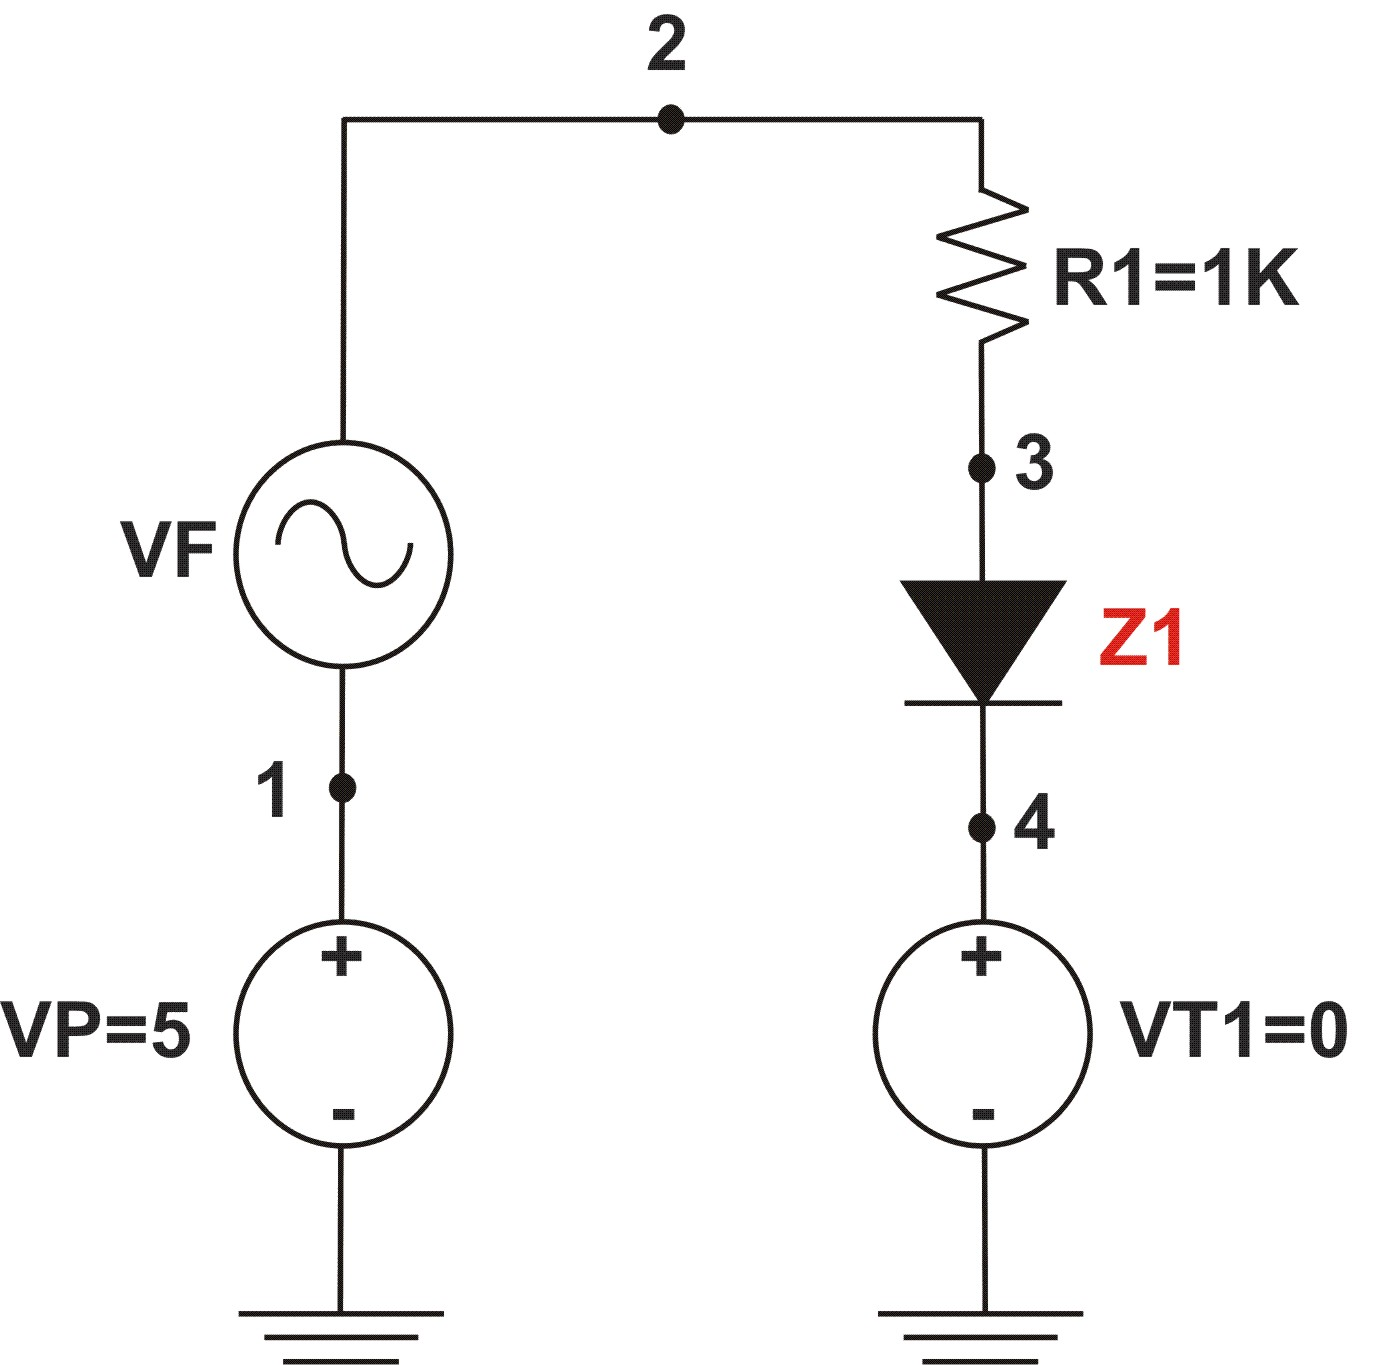
\includegraphics[width=2.300in,height= 2.270in]{diodeRegulatorSchem}}
  \caption[Voltage regulator schematic]{Voltage regulator schematic
The diode, Z1, is the PDE device in this example.\label{One_D_Diode_Schem}}
\end{figure}

\subsection{Netlist Explanation}
The model line for PDE devices serves only to set the level.  The default level
is 1, for a one-dimensional device.  Setting \texttt{level=2} will invoke
two-dimensional devices.  In this example, the level is not explicitly set, and
so \Xyce{} uses the default value which is 1.

The instance line is where most of the specific parameters are set for a
TCAD device.  In this example, the line appears as:

\texttt{YPDE Z1 3 4 DIODE na=1.0e17 nd=1.0e17 graded=1 l=5.0e-4 nx=101}

Doping parameters \texttt{na} and \texttt{nd} represent the
majority carrier doping levels on the N- and the P-sides of the
junction, respectively.  \texttt{graded=1} is also a doping parameter, and
specifies that the junction is a graded junction, rather than an abrupt
step-function junction.  \texttt{l=5.0e-4} specifies the length of
the device, in cm.  \texttt{nx=101} specifies that there are
101 mesh points, including the two endpoints.  For the one-dimensional
device, the mesh is always uniform, so the size of 
each mesh cell, $\Delta x$ will be:
\begin{equation}
  \Delta x = \frac{l}{nx-1} = \frac{\mbox{5.0e-4 cm}}{\mbox{100}} = \mbox{5.0e-6 cm}
\end{equation}
The mesh points $i=0 - 100$ will have the following locations, $x_{i}$:
\begin{eqnarray*}
  x_{i}   &=& i \Delta x\\
  x_{o}   &=& \mbox{0.0 cm} \\
  x_{1}   &=& \mbox{5.0e-6 cm} \\
  x_{2}   &=& \mbox{10.0e-6 cm} \\
          &\vdots& \\
  x_{100} &=& \mbox{5.0e-4 cm}
\end{eqnarray*}

\subsection{Boundary Conditions and Doping Profile}
The cited netlist example relies mostly on default parameters; therefore, it 
specifies nothing about electrodes, or boundary conditions, and has a minimal 
doping specification. A one-dimensional device can have only two electrodes 
connected to the circuit. The electrodes are at opposite ends of the domain, 
one at the first mesh point (\texttt{x=0.0 cm}, \texttt{i=0}) 
and the other at the opposite end of the domain, at the last mesh point 
(\texttt{x=5.0e-4 cm}, \texttt{i=101}).

The electrode associated with the first mesh point (\texttt{x=0.0 cm}) 
is connected to the \emph{second} circuit node on the instance line, 
while the electrode associated with the last mesh point (\texttt{x=l}) 
is connected to the \emph{first} circuit node on the instance line.  
For the doping used in this example, the junction is in the exact 
center of the device (\texttt{x=l/2}), and the n-side
is the region defined by \texttt{x<l/2}, and the p-side is the region defined by
\texttt{x>l/2}.  This default doping, along with the electrode-circuit connectivity,
results in a one-dimensional device that behaves like a traditional
SPICE-style diode.  For a complete discussion of how to specify
a doping profile see section~\ref{Manual_Doping}.  For a complete discussion
of how to specify electrodes (including boundary conditions), see
section~\ref{PDE_Electrode}.

\subsection{Results}
Figure~\ref{One_D_outputSignal} shows the transient behavior of this circuit.  
The voltage drop across the diode (V(3)) is nearly the same for a wide 
range of currents, and is nearly constant.  The
voltage drop (V(2)-V(3)) across the series resistor, \texttt{R1}, is much more
sensitive, and so most of the voltage 
variation of the input sine wave is accounted for by \texttt{R1}.
% Output Signal.
\begin{figure}
\begin{minipage}[b]{0.5\linewidth}
\centering
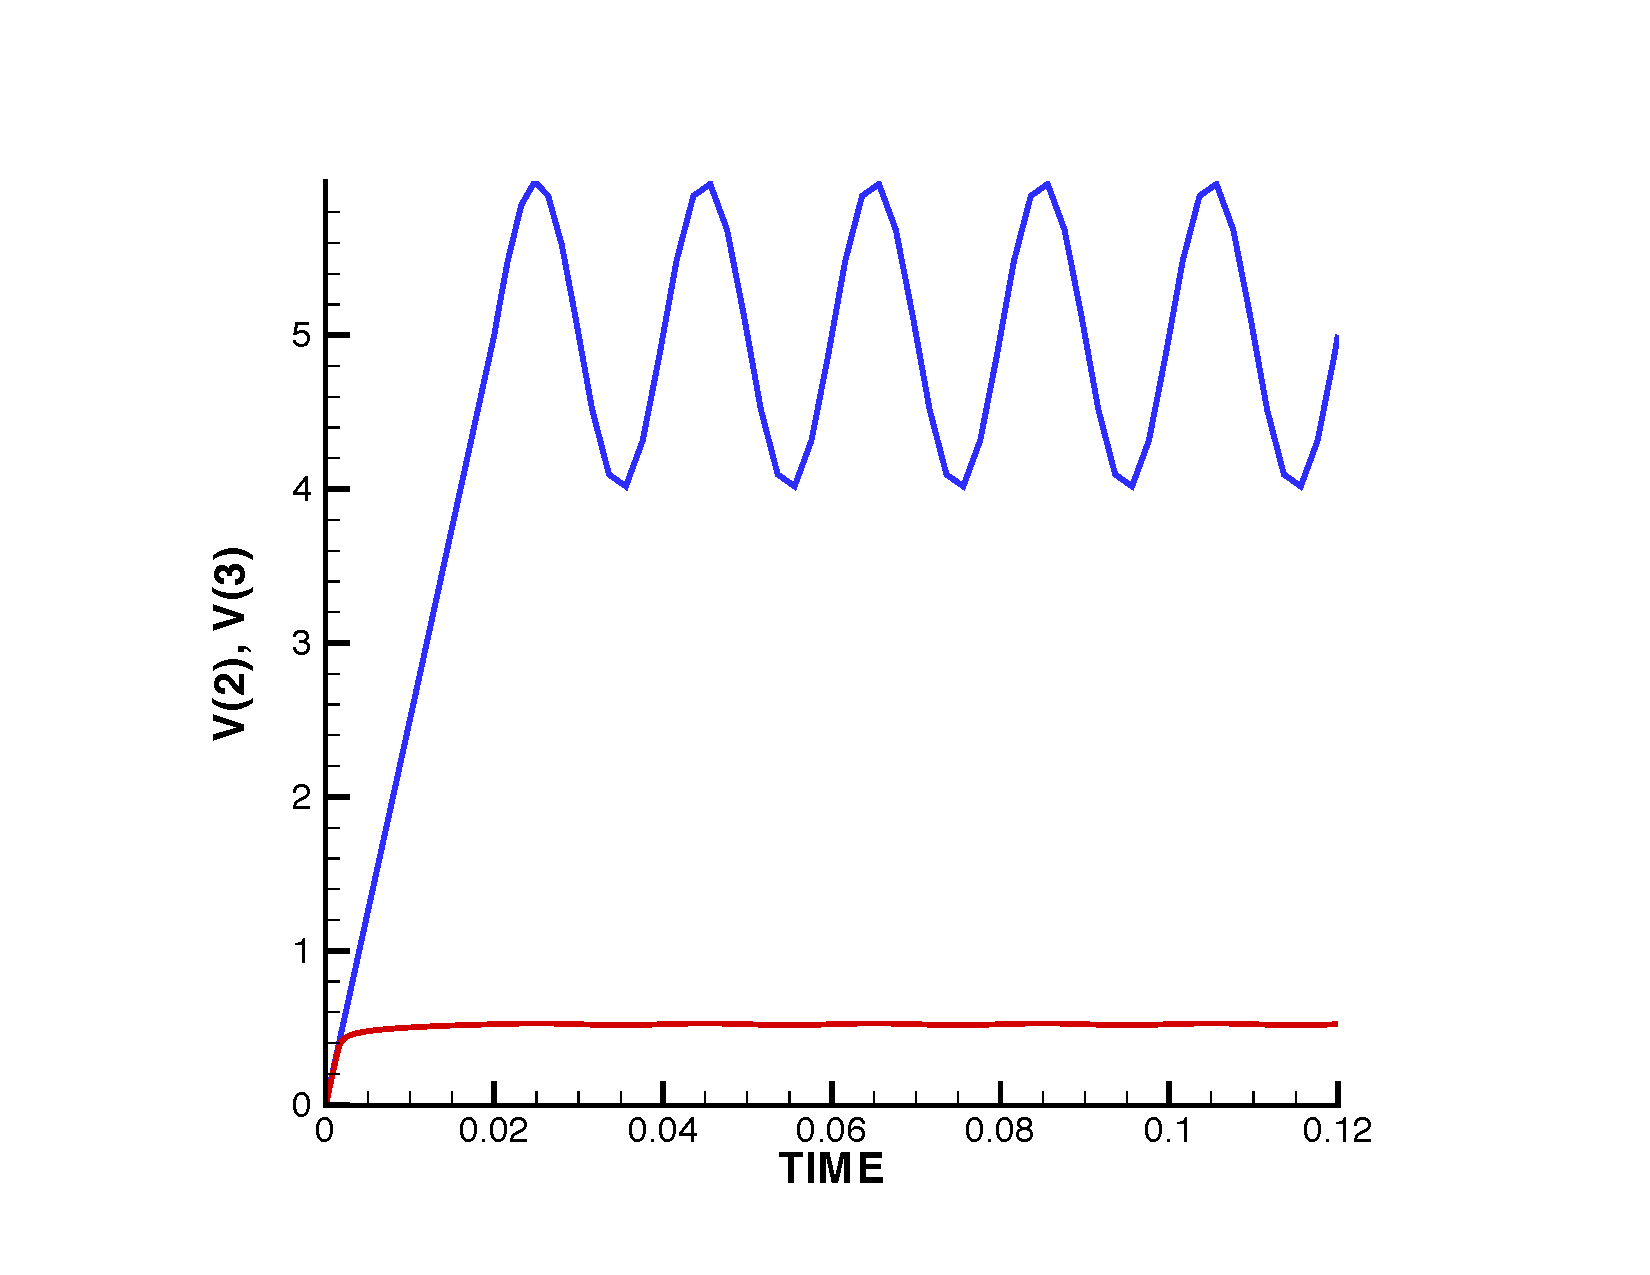
\includegraphics[scale=0.4]{Z1_trans}
\end{minipage}
\hspace{0.5cm}
\begin{minipage}[b]{0.5\linewidth}
\centering
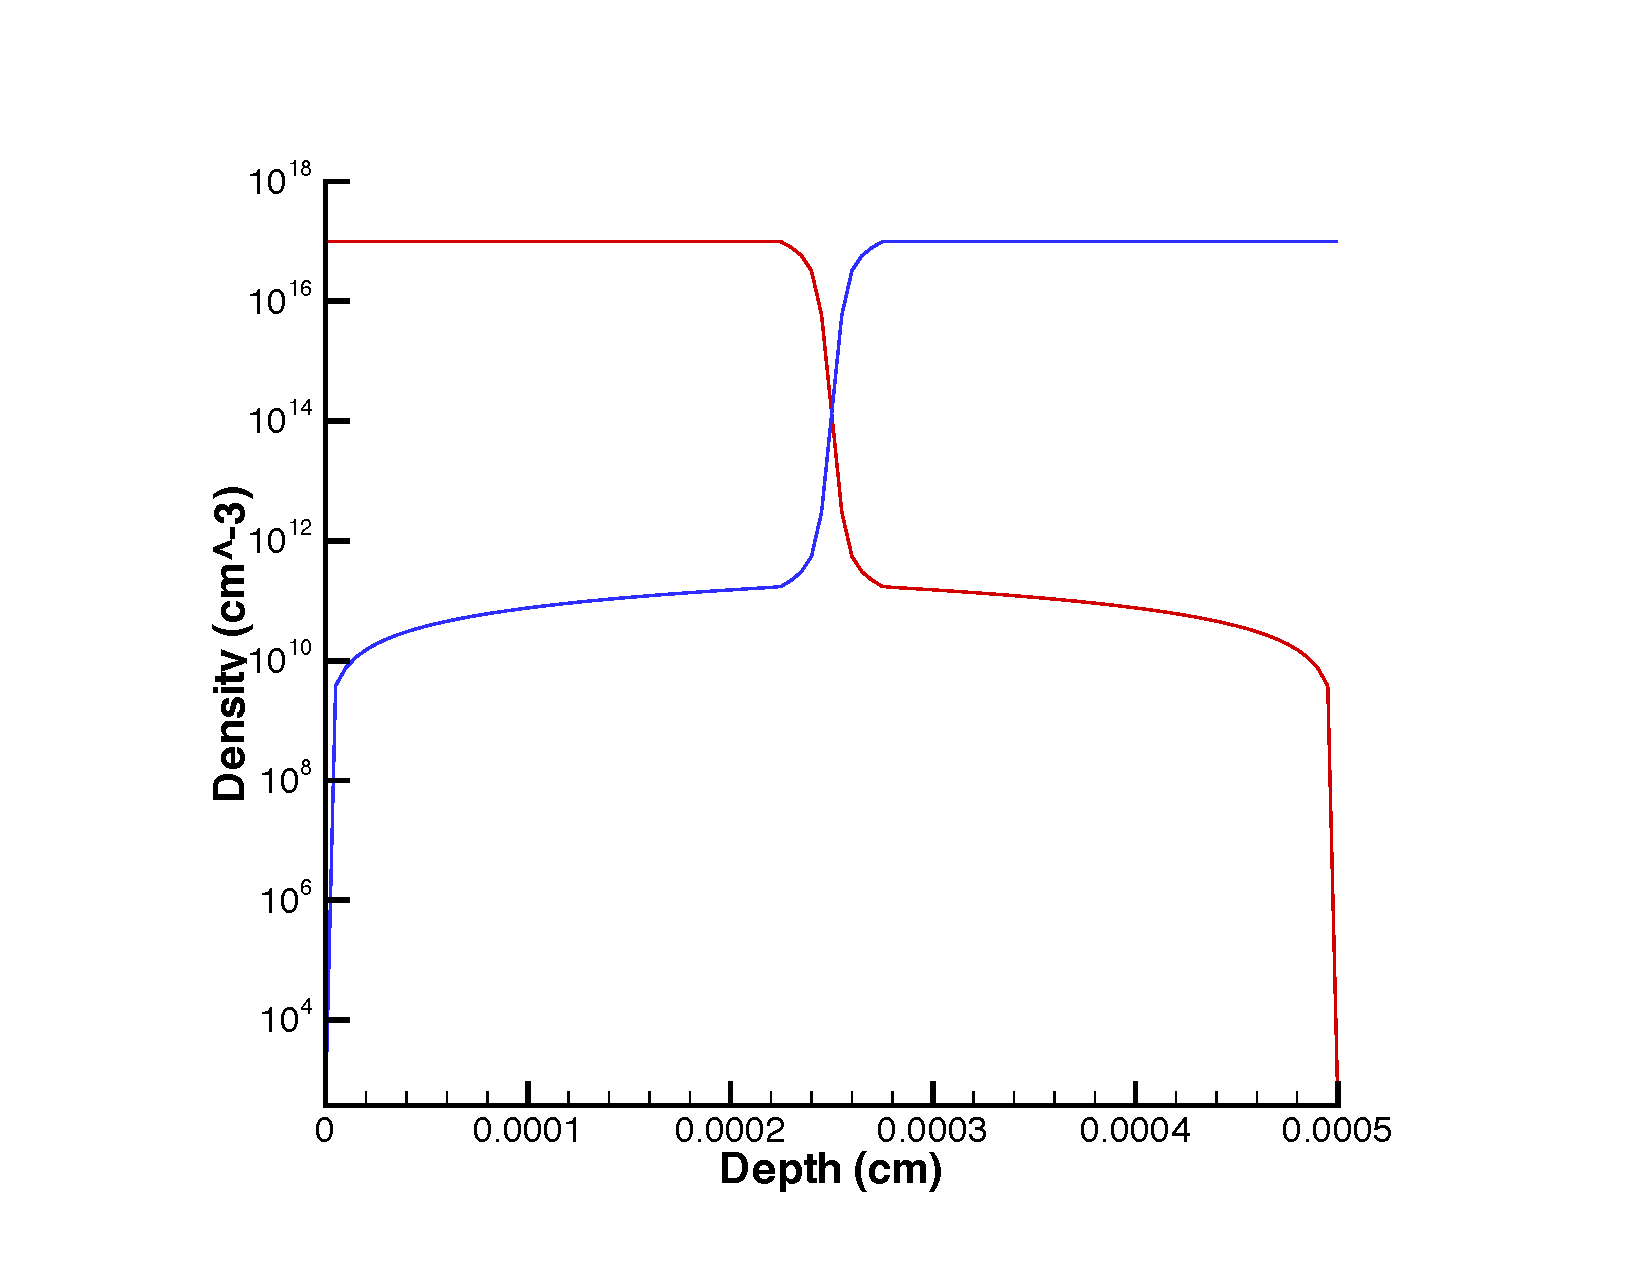
\includegraphics[scale=0.4]{Z1_dens}
\end{minipage}
\caption[Results for voltage regulator]{Results for voltage regulator.  In the left plot, the transient output is shown, in which the input voltage is blue and the output voltage is red.  In the right plot, the initial carrier densities are shown, with the electron density in red and the hole density in blue.}
\label{One_D_outputSignal}
\end{figure}

\section{Two-Dimensional Example} \label{PDE_Two_D_Example}
Figure~\ref{Two_D_BJT_Netlist} presents an example netlist for a simulation of 
a two-dimensional bipolar transistor.   As before, the PDE device instance line 
is in red, while the PDE device model line is in blue.  In this case, note that 
the model line specifies the level, which is set to 2.  This is required for the 
two-dimensional device.  This particular example is a DC sweep of a bipolar 
transistor device. Figure~\ref{twoD_BJT_Schem} presents a schematic illustrating 
this circuit.
% two dimensional netlist example
\begin{figure}
  \begin{centering}
    \shadowbox{
      \begin{minipage}{0.8\textwidth}
        \begin{vquote}
Two-Dimensional Example
VPOS  1 0 DC 5V
VBB   6 0 DC -2V
RE    1 2 2K
RB    3 4 190K

\color{XyceRed} YPDE BJT 5 3 7 PDEBJT meshfile=internal.msh 
+ node = \{name = collector, base, emitter\}
+ tecplotlevel=2 txtdatalevel=1
+ mobmodel=arora
+ l=2.0e-3  w=1.0e-3
+ nx=30     ny=15 
\color{XyceDarkBlue}.MODEL PDEBJT   ZOD  level=2 \color{black}

* Zero-volt sources acting as an ammeter to measure the
* base, collector, and emmitter currents, respectively
VMON1 4 6 0
VMON2 5 0 0
VMON3 2 7 0 

.DC VPOS 0.0 12.0 0.5 VBB -2.0 -2.0 1.0
.options NONLIN maxstep=70 maxsearchstep=1 
+ searchmethod=2 
.options TIMEINT reltol=1.0e-3 abstol=1.0e-6 
+ firstdcopstep=0 lastdcopstep=1
.PRINT DC V(1) I(VMON1) I(VMON2) I(VMON3)
.END
\end{vquote}

\end{minipage}
}
\caption[Two-dimensional BJT netlist]
{Two-dimensional BJT netlist.  Figures~\ref{twoD_BJTResA} and~\ref{twoD_BJTResB} provide some of the results of this netlist.\label{Two_D_BJT_Netlist}}
\end{centering}
\end{figure}
% BJT Circuit Schematic
% Original dimensions of picture: w=5.62 h=7.35 (inches)
\begin{figure}
  \centering
  \scalebox{0.5}
  {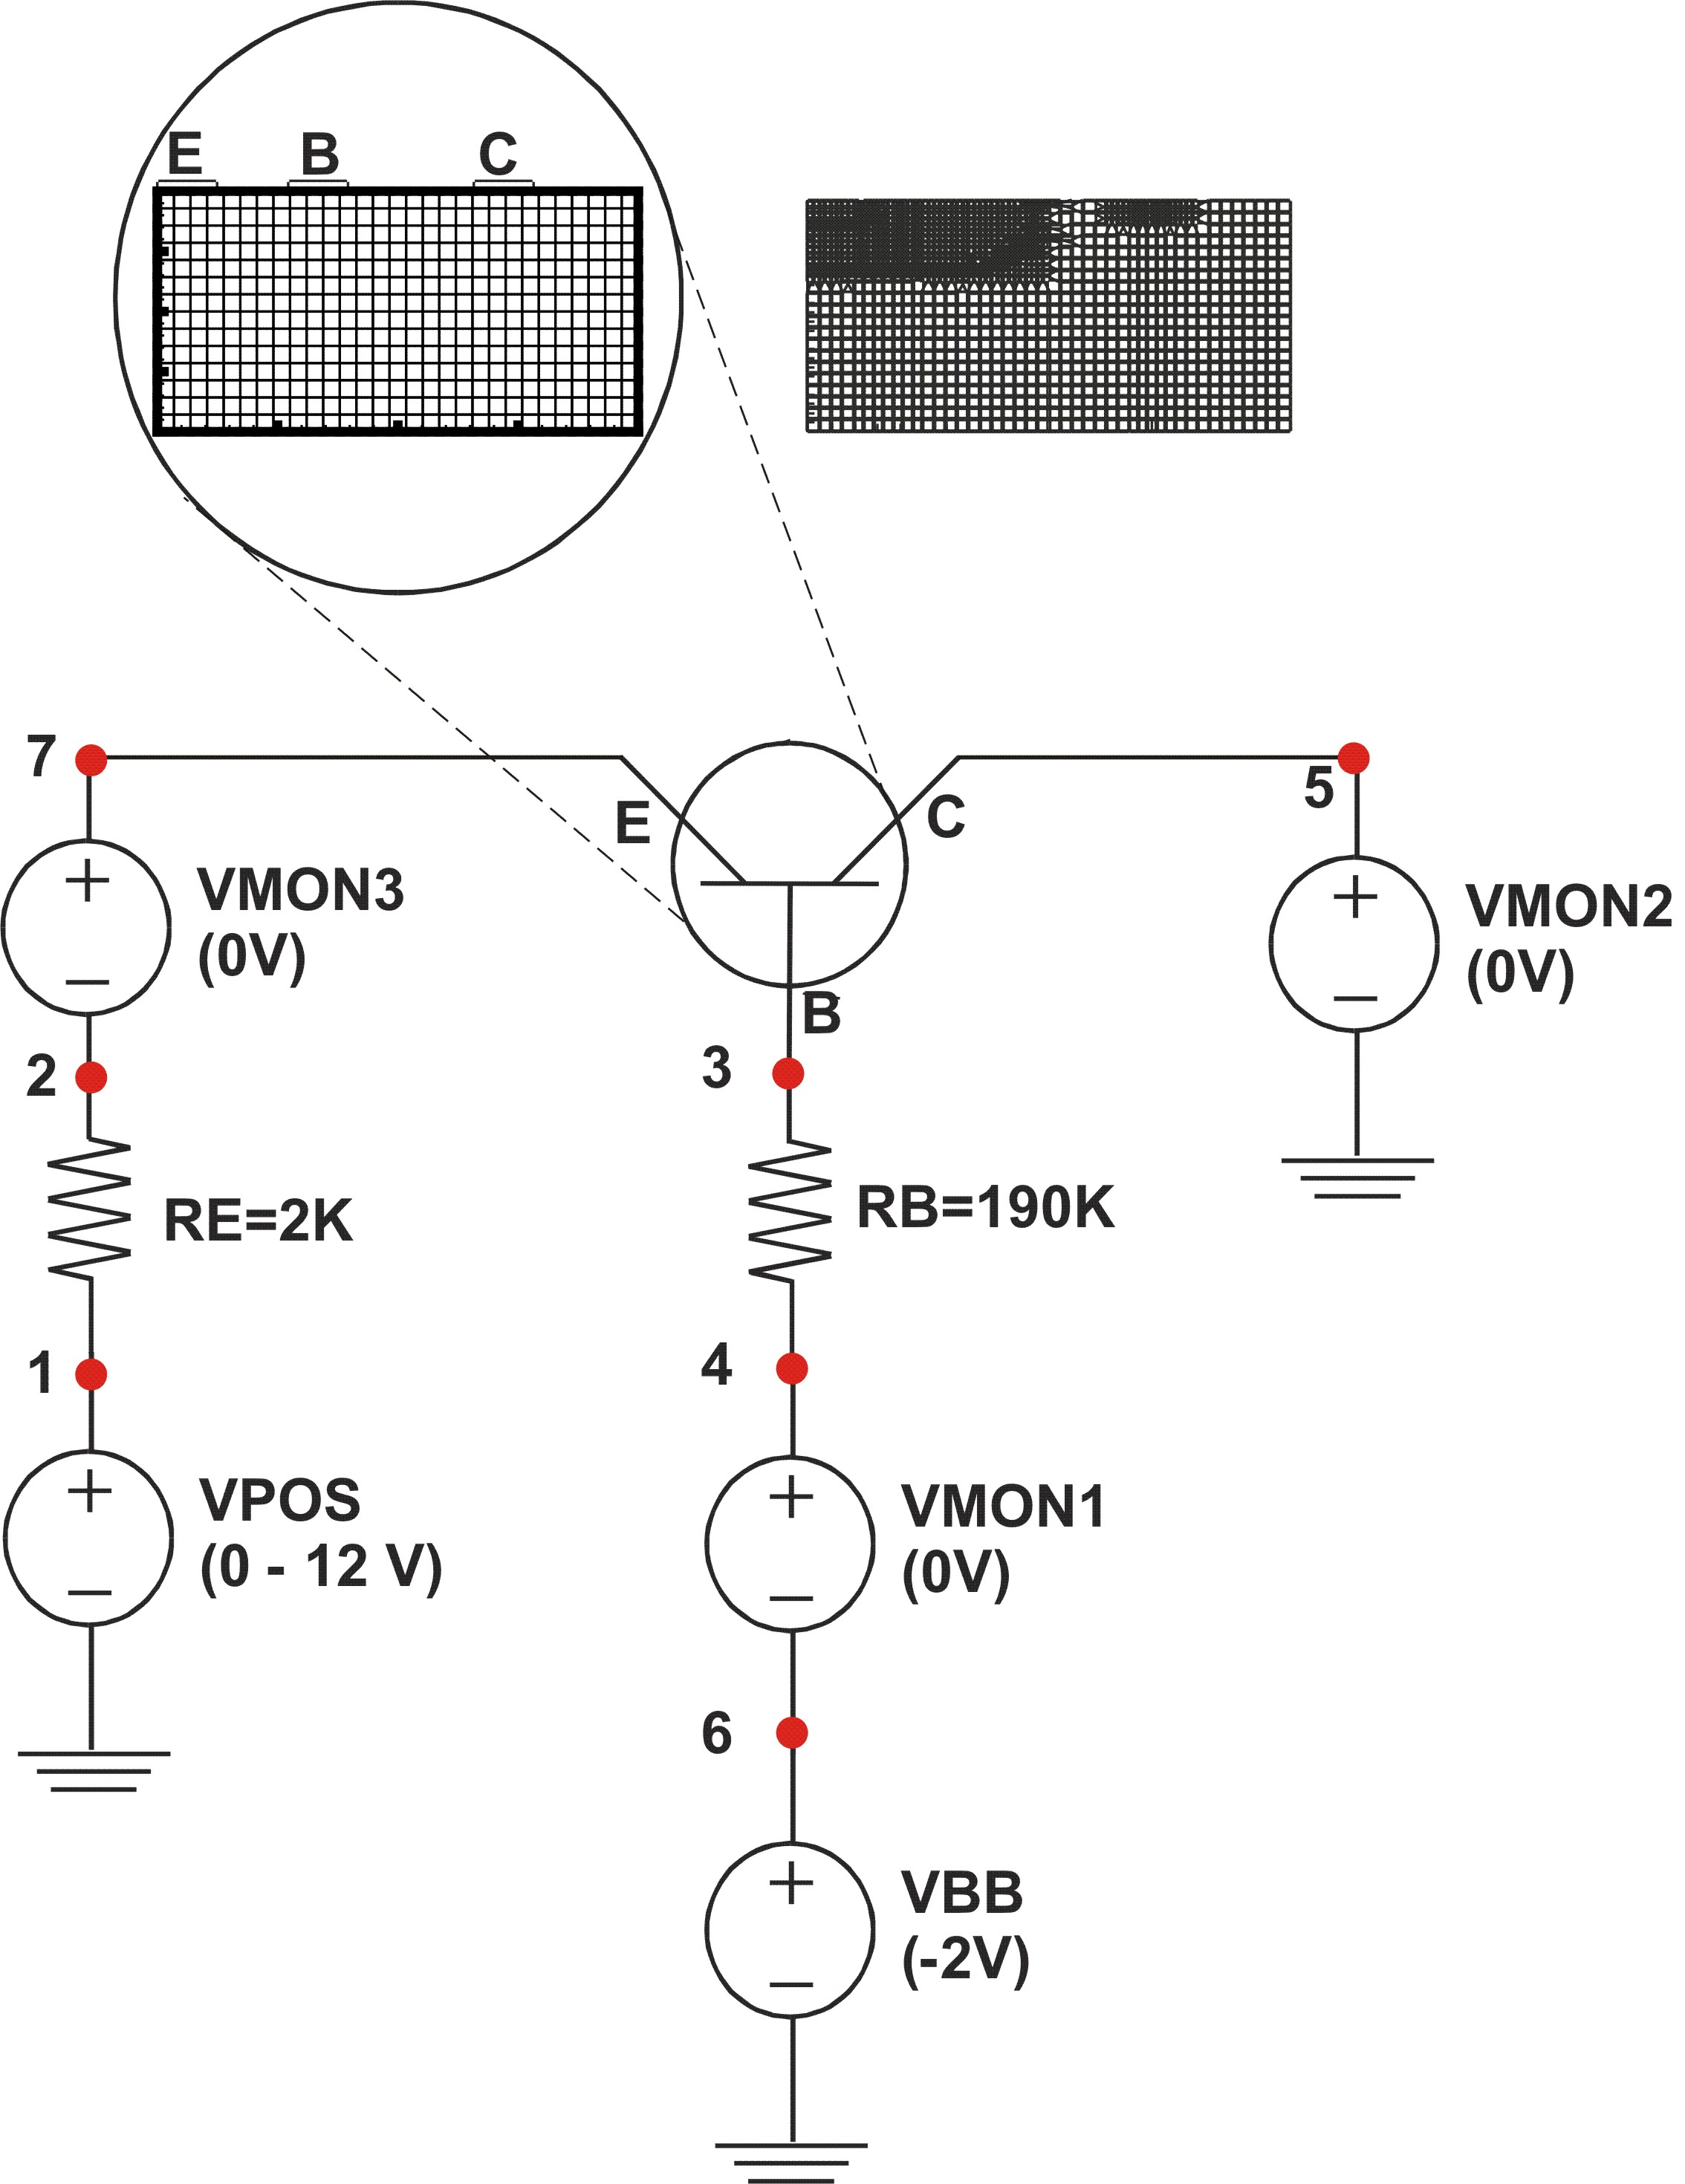
\includegraphics[]{twoDcircuit}}
  \caption[Two-dimensional BJT circuit schematic]
  {Two-dimensional BJT circuit schematic This schematic is for the circuit described by the netlist in figure~\ref{Two_D_BJT_Netlist}.  The mesh in the large circle is the mesh used in the example.  The other mesh, which contains some mesh refinement, is included in the figure as an example of what is possible with an external mesh generator.
\label{twoD_BJT_Schem}}
\end{figure}

\subsection{Netlist Explanation}
The two-dimensional device can have 2 to 4 electrodes.  In this example there
are three; nodes 5, 3, and 7, corresponding to the three names
on the ``node'' line,  which appears as:

\texttt{+ node = \{name = collector, base, emitter\} }

This line specifies that node 5 is connected to an electrode named 
``collector,'' node 3 is connected to an electrode named ``base,'' and node 7
is connected to an electrode named ``emitter''.    Although this example only
contains the electrode names, the ``node'' specification
can contain a lot of information. Section~\ref{PDE_Electrode} provides a full explanation of the
electrode parameters.  

The next line contains parameters concerned with plotting the results, and
appears as follows:

\texttt{+ tecplotlevel=2 txtdatalevel=1}

These are not related to the output specified by \texttt{.PRINT}, which outputs circuit data.  
The \texttt{tecplotlevel} command enables files to be output readable by Tecplot,  
which can then be used to create contour plots of 
quantities such as the electron density, electrostatic potential and the
doping profile.  Figures~\ref{twoD_BJTResA} and~\ref{twoD_BJTResB} 
contain examples of Tecplot-generated contour plots, which were generated
from the results of this example.

The \texttt{txtdatalevel} command enables a text file with volume averaged
information to be output to a file.  \Xyce{} will update both of 
these output files at each time step or DC sweep step.

The next line, \texttt{mobmodel=arora}, specifies which mobility model to
use.  Section~\ref{PDE_Mobility} provides for more detail on available mobility models.

The last two lines, specify the mesh of the device, and are given by:

\texttt{+ l=2.0e-3  w=1.0e-3} \\
\texttt{+ nx=30     ny=15}

This numbers are used in nearly the same way as the one-dimensional case used the \texttt{l} and
\texttt{nx} parameters.  The mesh is Cartesian, and the spacing is uniform.  

\subsection{Doping Profile}
As in the one-dimensional example, the two-dimensional example in figure
~\ref{Two_D_BJT_Netlist} specifies nothing about the doping profile, and thus 
relies on default settings.  In this case there are three specified electrodes, 
which by default results in the doping profile of the bipolar junction transistor (BJT).  
Section~\ref{PDE_Doping} provides a complete description of how to specify a 
doping profile, and describes the various default impurity profiles.

\subsection{Boundary Conditions and Electrode Configuration}
As in the one-dimensional example, the two-dimensional example in
figure~\ref{Two_D_BJT_Netlist} specifies nothing about
the electrode configuration or the boundary conditions, and relies on
default settings.  To be consistent with the default three-terminal doping,
the device has terminals that correspond to that of a BJT.  All three
electrodes (collector, base, emitter) are along the top of the device.

By default all electrodes are considered to be neutral contacts.  The 
boundary conditions applied to the electron density, hole density, and 
electrostatic potential are all Dirichlet conditions.

Section~\ref{PDE_Electrode} discusses how to specify electrodes in detail 
(including boundary conditions).

\subsection{Results}
Figures~\ref{twoD_BJTResA}, ~\ref{twoD_BJTResB} and ~\ref{twoD_BJTResC} provide 
results for the two-dimensional example.  The first two figures are contour plots 
of the electrostatic potential.  The first corresponds to the first DC sweep step, 
where VPOS is set to 0.0 Volts.  The second corresponds to the final DC sweep 
step, in which VPOS has a value of 12.0 volts.  The voltage source, VPOS, 
applies a voltage to the emitter load resistor, RE, so some of the 12.0V is 
dropped across RE, an the rest is applied to the BJT.

The third figure is an I-V curve of the dependence of the three terminal currents 
on the applied emitter voltage.  For the entire sweep, $-2.0$ V has been applied to 
the base load resistor and, as this transistor is a PNP transistor, this results 
in the transistor being in an ``on'' state.  The emitter-collector current varies 
nearly linearly with the applied emitter voltage. Also, as can be expected 
because of current conservation, the three currents sum to nearly zero.

Note that the mesh used to generate these results is visible in 
figure~\ref{twoD_BJTResA}, and was generated using the internal ``uniform mesh''.  
This mesh will not produce a very accurate result, as it does not 
resolve the depletion regions very well.  Accuracy can often be improved 
using mesh refinement near the depletion regions.  However, such meshes must be 
read in from an external mesh generator, which currently has limited support
as a alpha-level capability.

% BJT steady state, initial step.
\begin{figure}
  \centering
  \scalebox{1.0}
  {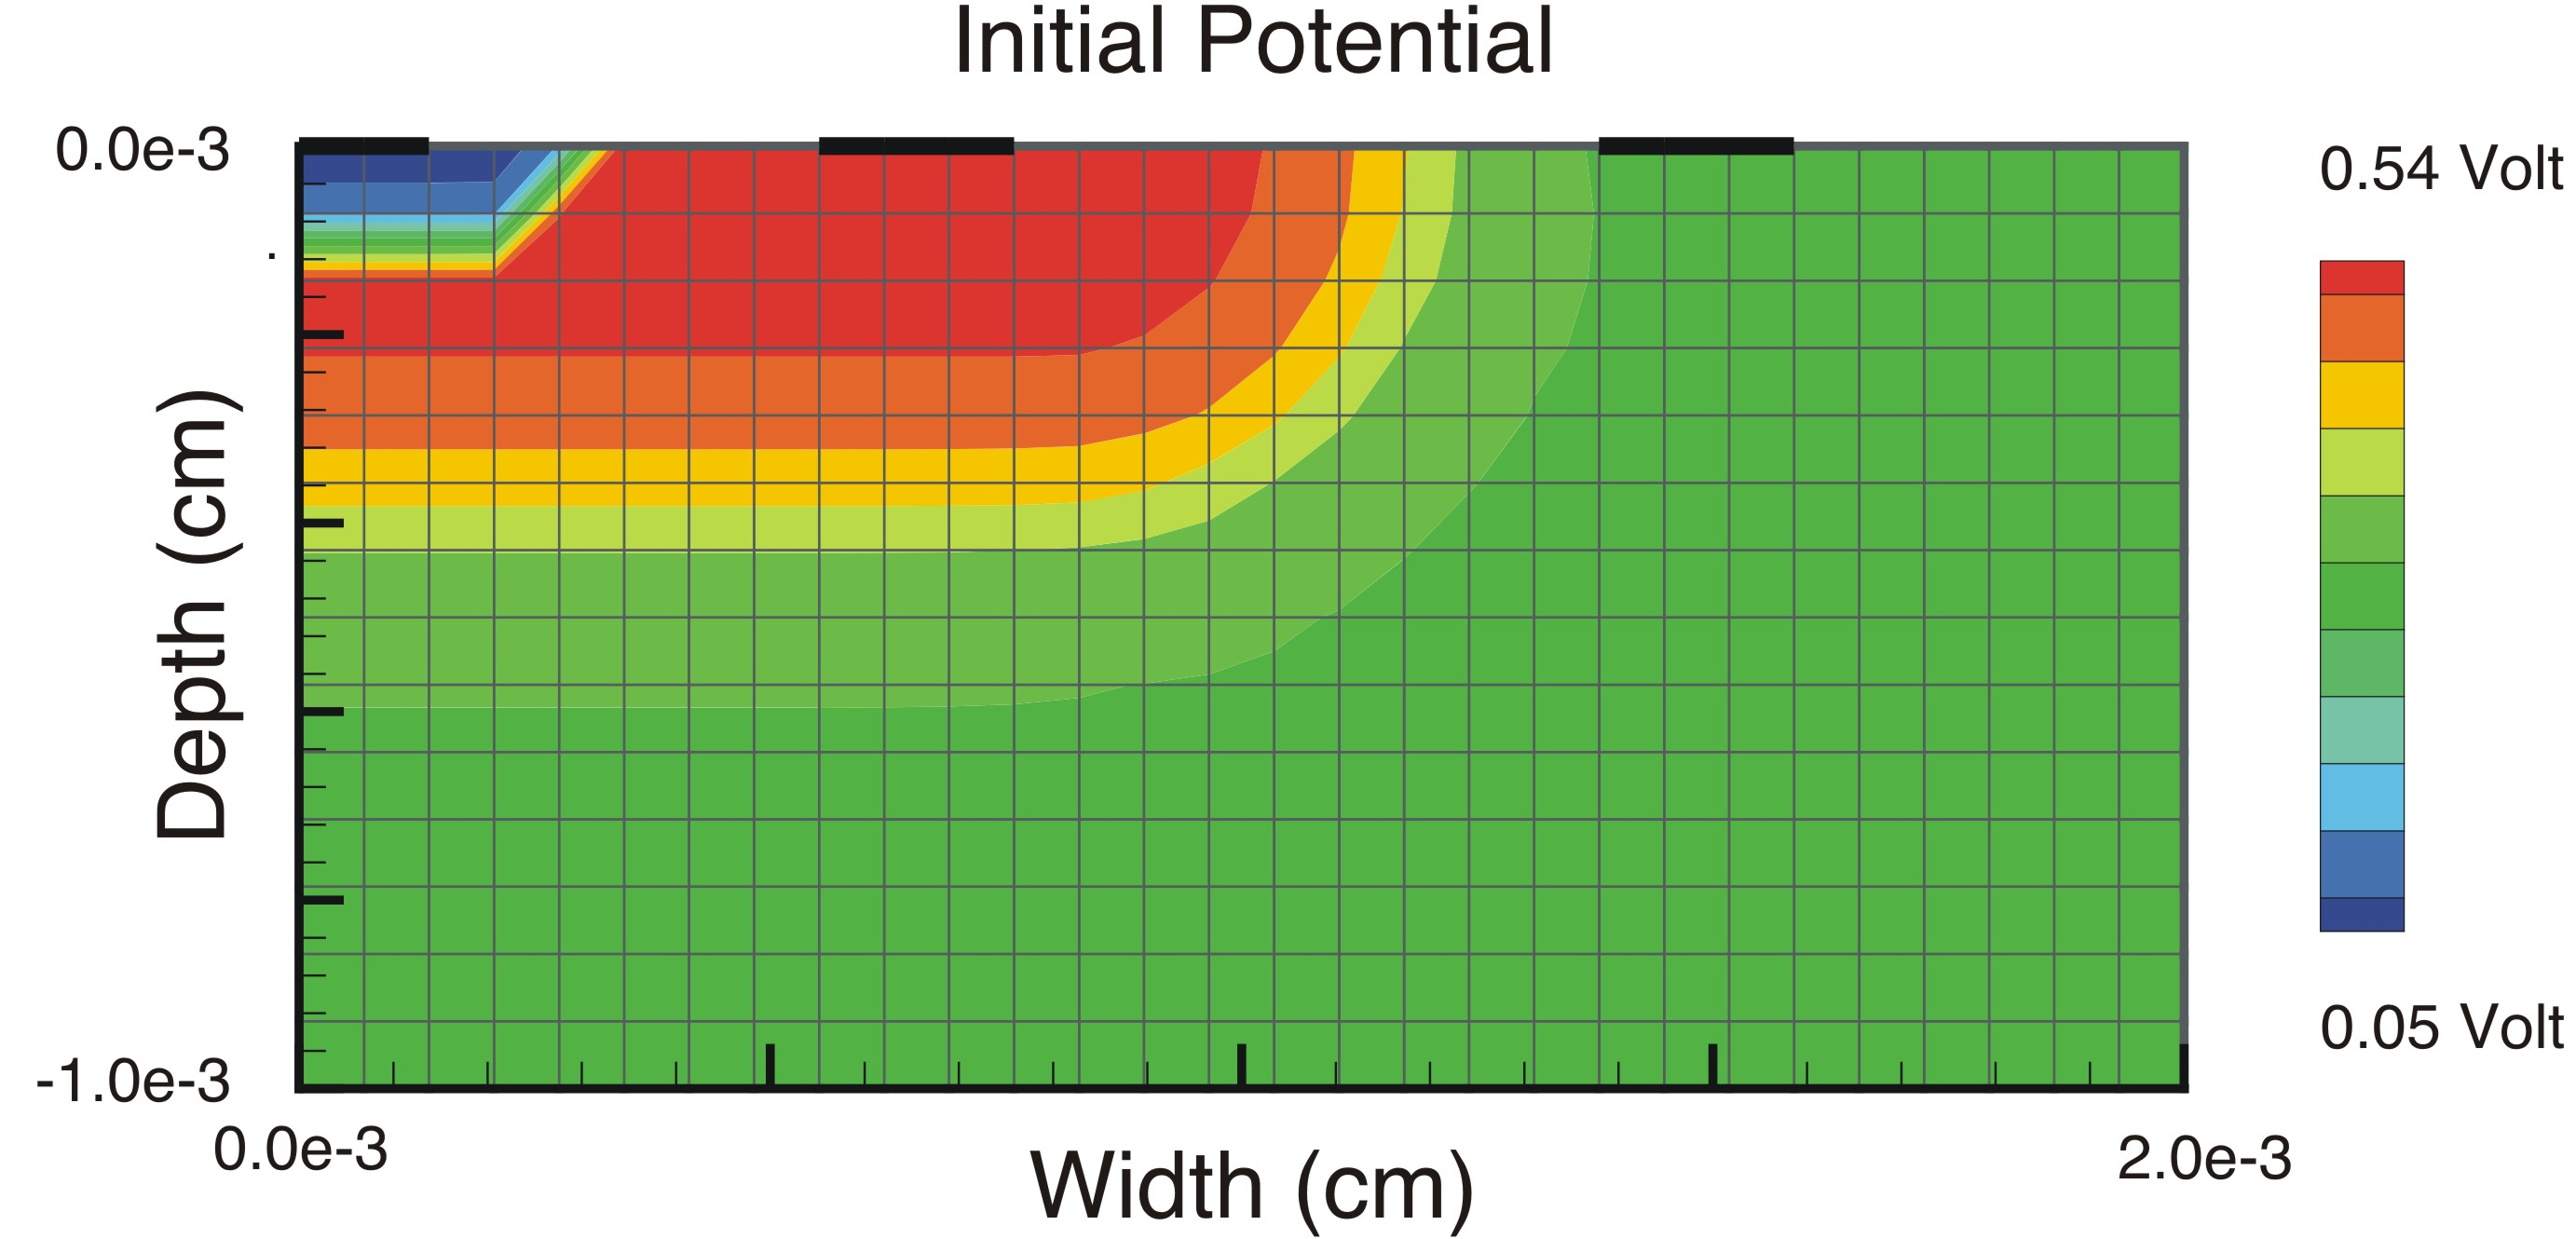
\includegraphics[width=4.610in,height= 2.165in]{twoDresultA}}
  \caption[Initial two-dimensional BJT result]
  {Initial two-dimensional BJT result
A Tecplot-generated contour plot of the electrostatic potential at the first DC 
  sweep step of the netlist in figure~\ref{Two_D_BJT_Netlist}.  
\label{twoD_BJTResA}}
\end{figure}

% BJT steady state, final step.
\begin{figure}
  \centering
  \scalebox{1.0}
  {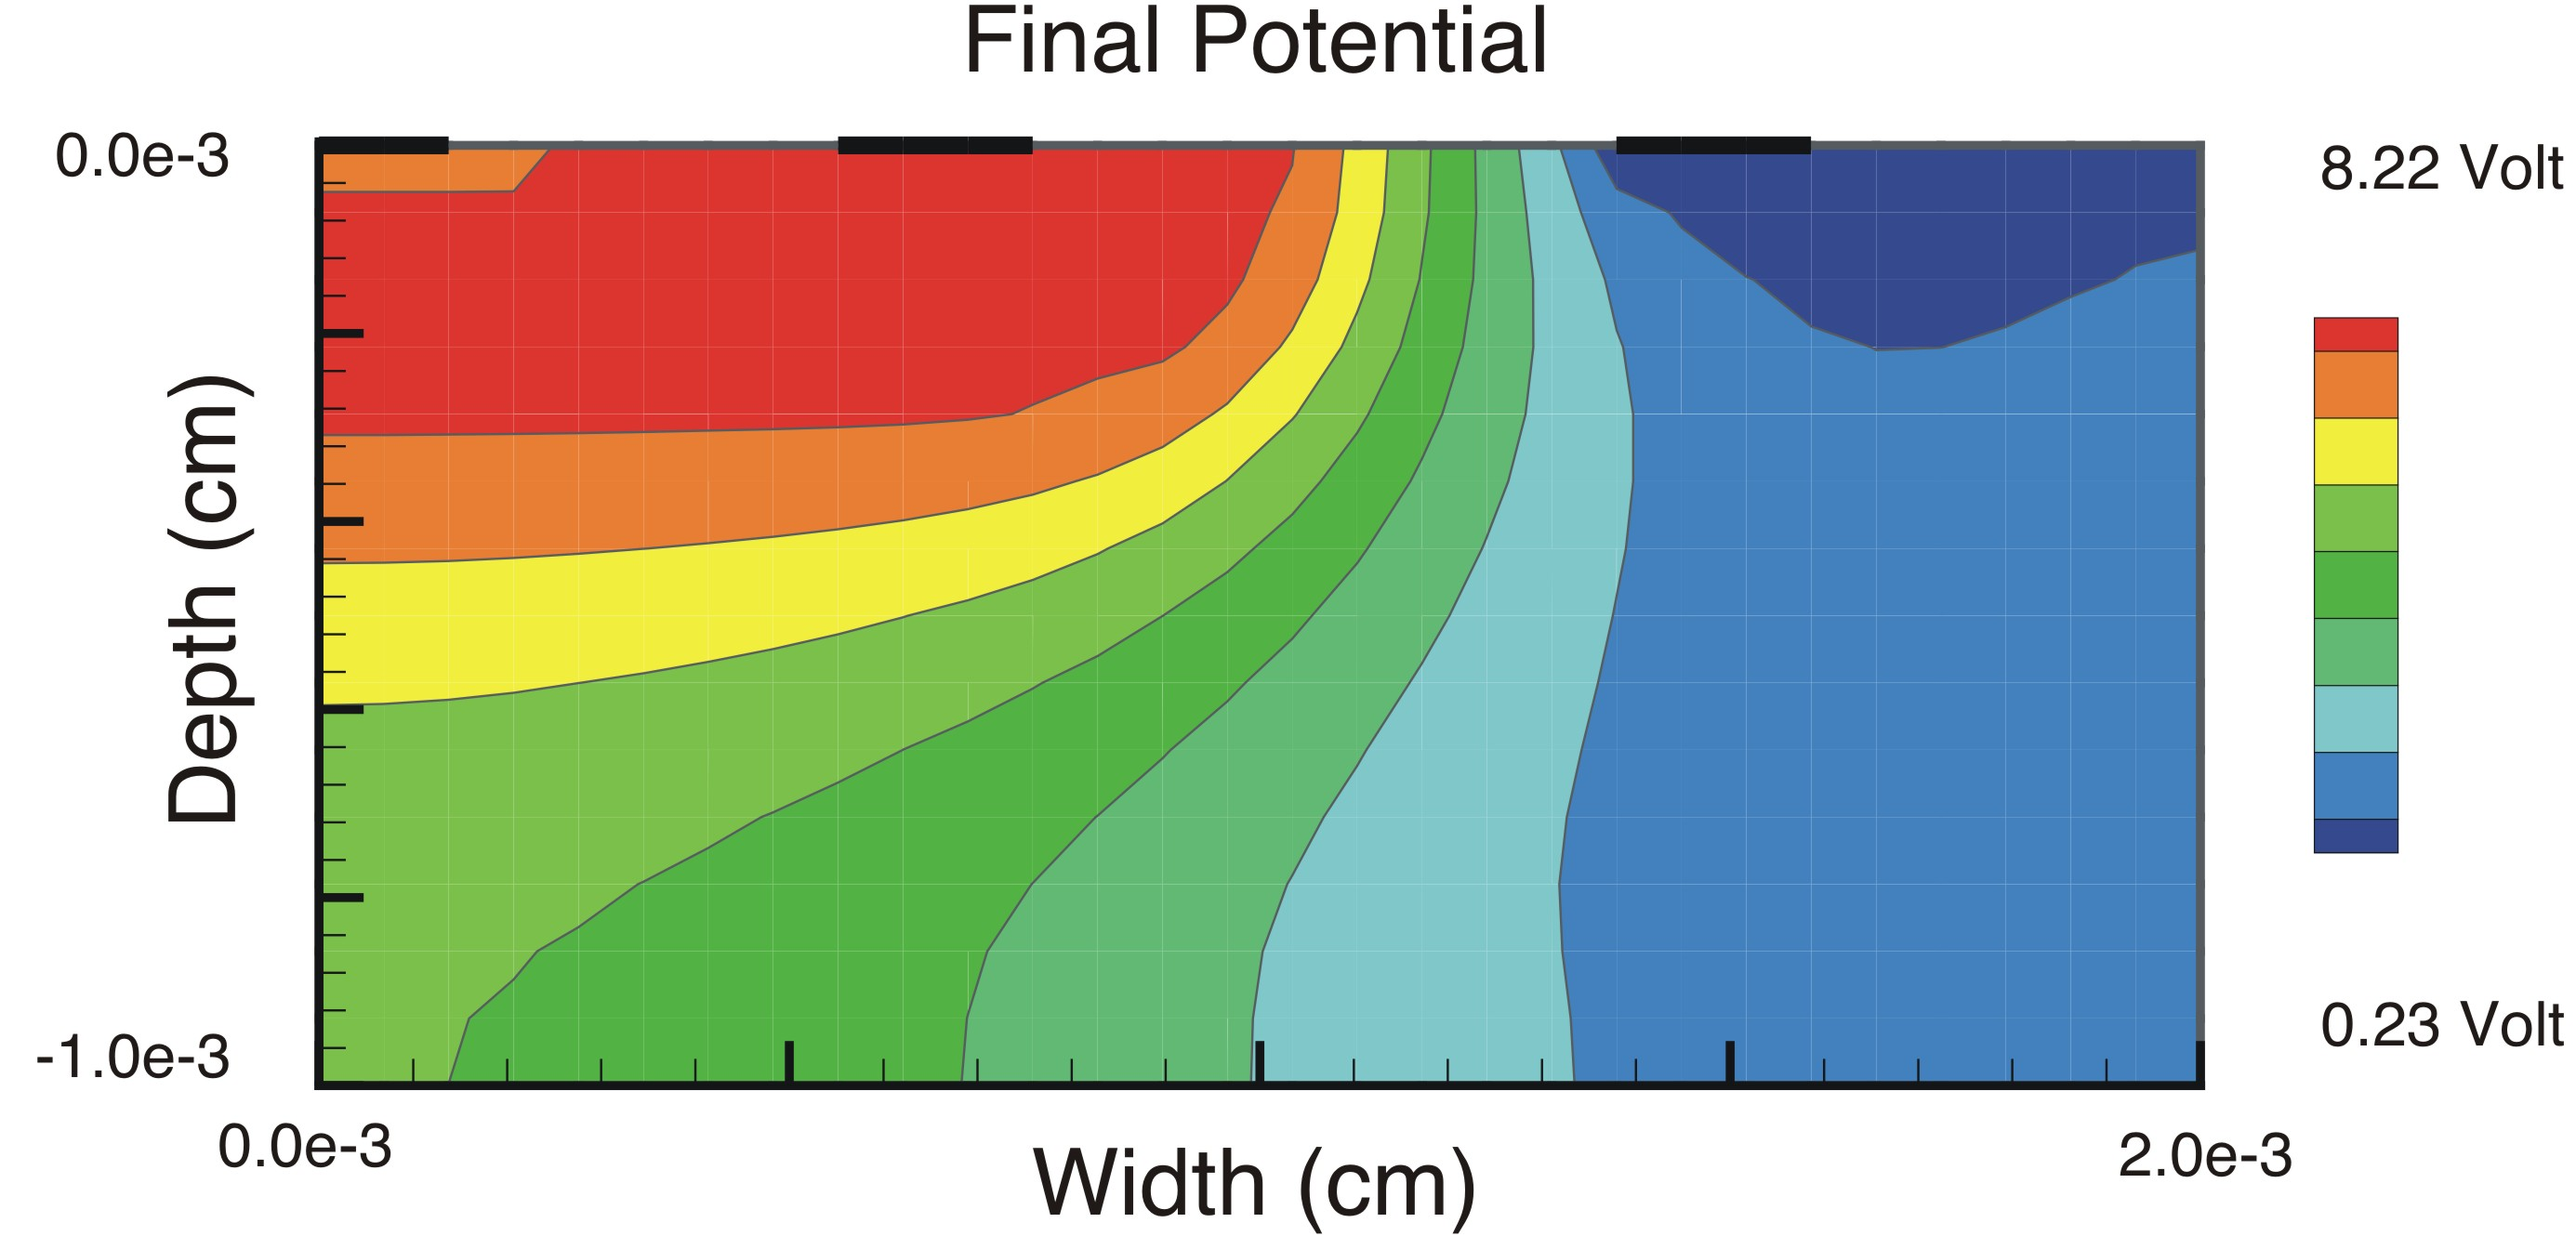
\includegraphics[width=4.610in,height= 2.165in]{twoDresultB}}
  \caption[Final two-dimensional BJT result.]
  {Final two-dimensional BJT result.  
A Tecplot-generated contour plot of the electrostatic potential at the last DC sweep 
  step of the netlist in figure~\ref{Two_D_BJT_Netlist}.  
\label{twoD_BJTResB}}
\end{figure}

% BJT steady state, I-V curve.
\begin{figure}
  \centering
  \scalebox{0.5}
  {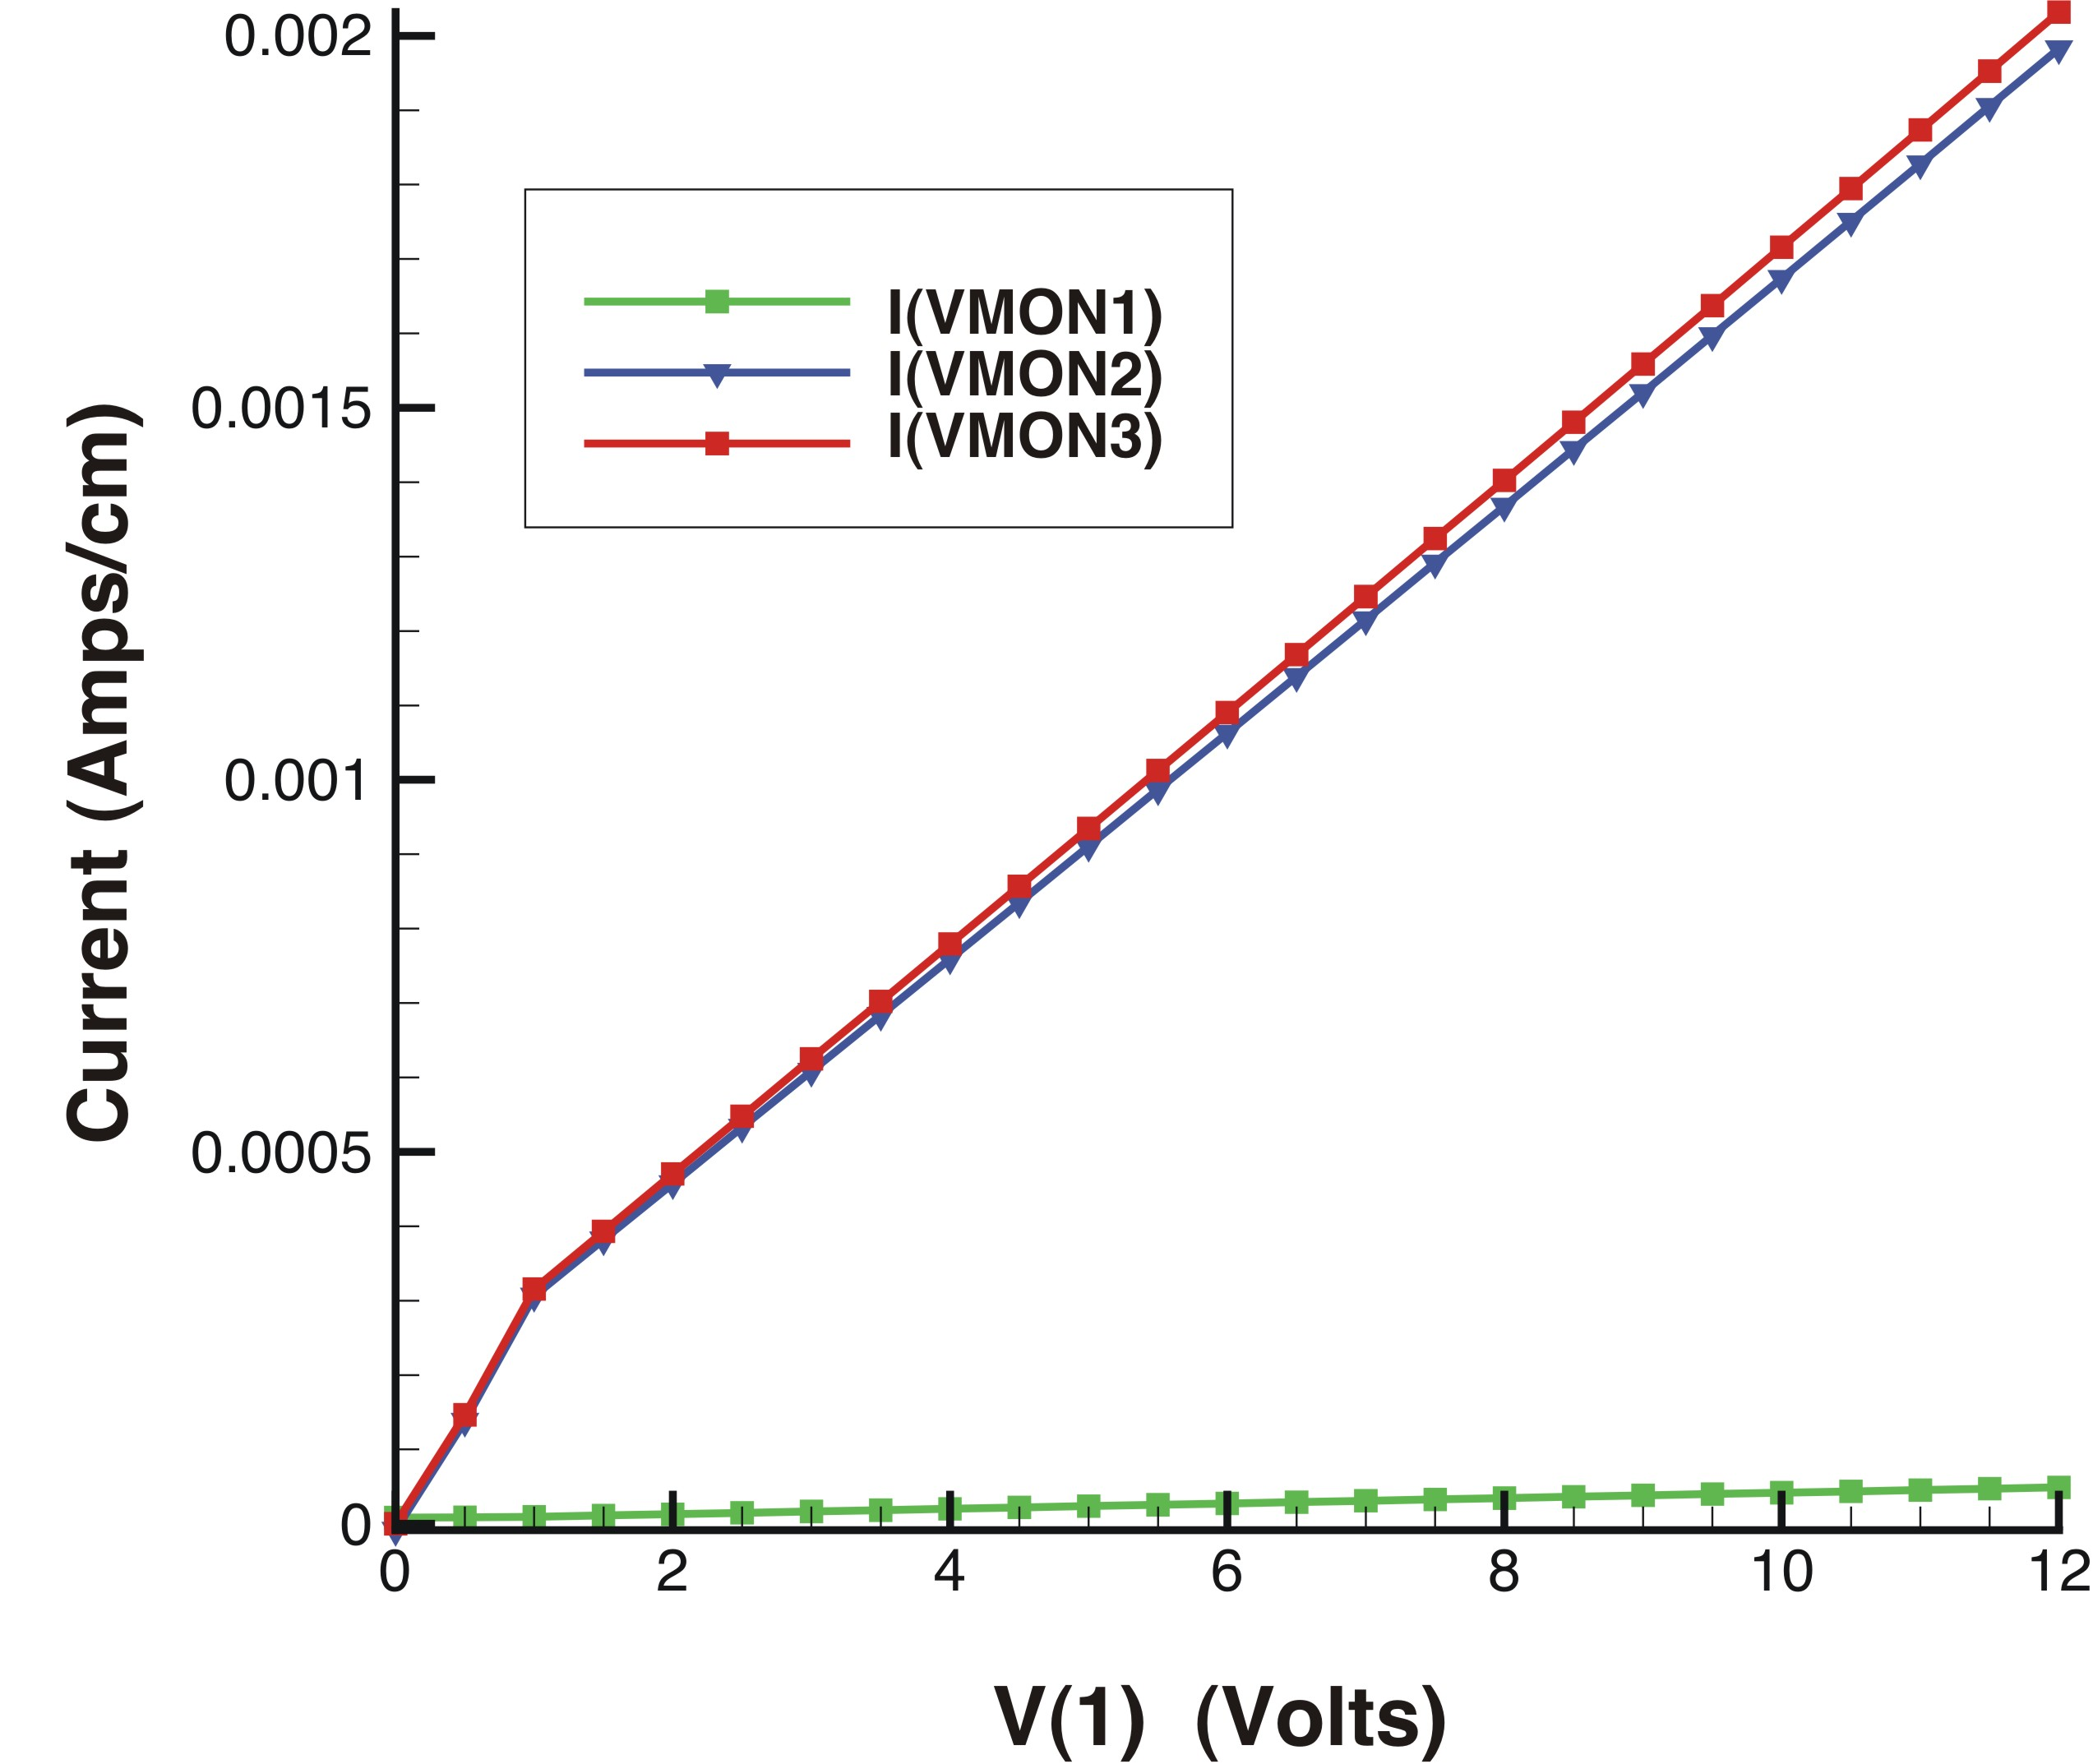
\includegraphics[]{twoDresultC}}
  \caption[I-V two-dimensional BJT result for the netlist in figure~\ref{Two_D_BJT_Netlist}]
  {I-V two-dimensional BJT result for the netlist in figure~\ref{Two_D_BJT_Netlist}.  
The three plotted currents are through the three BJT electrodes, and as expected they add (if corrected for sign) to zero.  I(VMON1) is the base current, I(VMON2) the collector current, and I(VMON3) the emitter current.  V(1) is the voltage applied to the emitter load resistor, RE.  
\label{twoD_BJTResC}}
\end{figure}

\section{Doping Profile} \label{PDE_Doping}
\Xyce{} used default doping profiles in the two examples from the previous section, so no doping parameters were 
specified.  Default profiles are uniquely specified by the number
of electrodes.  In practice, especially for two-dimensional simulations, the user will generally need to specify the doping profile manually.

\subsection{Manually Specifying the Doping} \label{Manual_Doping}
Figure~\ref{One_D_Doping_Electrode_1} shows a circuit netlist for a one-dimensional device with 
a detailed, manual specification of the doping
profile.  Figure~\ref{Two_D_Doping_Electrode_1} illustrates a similar, two-dimensional version of this problem. For this
discussion, the one-dimensional example will be referred to, but the information conveyed is equally applicable to the two-dimensional case.

In both examples, the parameters associated with doping are in red text.  The doping is specified with one or
more regions, which are summed together to obtain the total profile.  Doping regions are specified in a tabular format, with each column
representing a different region.  

\begin{figure}
  \begin{centering}
    \shadowbox{
      \begin{minipage}{0.8\textwidth}
        \begin{vquote}

\color[gray]{0.5}Doping and Electrode specification example
vscope   0   1   0.0
rscope   2   1   50.0
cid      3   0   1.0u
r1       4   3   1515.0
vid      4   0   5.00 \color{black}
YPDE Z1DIODE 2 3 PDEDIODE nx=301 l=26.0e-4 
\color{XyceRed}* DOPING REGIONS:    region 1,  region 2,   region 3
+ region= \{name     =    reg1,      reg2,  reg3
+          function = uniform,  gaussian,  gaussian
+          type     =   ntype,     ptype,     ntype
+          nmax     = 4.0e+12,   1.0e+19,   1.0e+18
+          nmin     = 0.0e+00,   4.0e+12,   4.0e+12
+          xloc     =    0.0 ,  24.5e-04,   9.0e-04
+          xwidth   =    0.0 ,   4.5e-04,   8.0e-04
+          flatx    =    0   ,        0 ,       -1 \}\color{black}
*--------end of  Diode PDE device ----------------\color[gray]{0.5}
.MODEL PDEDIODE  ZOD  level=1 
.options NONLIN maxsearchstep=1 searchmethod=2 
.options TIMEINT reltol=1.0e-3 abstol=1.0e-6 
.DC vscope 0 0 1
.print DC v(1) v(2) v(3) v(4) I(vscope) I(vid)
.END
\end{vquote}
\end{minipage}
}
\caption{One-dimensional example, with detailed doping
\label{One_D_Doping_Electrode_1}}
\end{centering}
\end{figure}

In the one-dimensional example, there are three regions, which are illustrated in
figure~\ref{Doping_Profile_1D}.  Region 1 is a uniform n-type
doping, with a constant magnitude of \texttt{4.0e+12} donors per cubic cm.  This 
magnitude is set by the parameter \texttt{nmax}.  As the
doping in this region is spatially uniform, the only meaningful parameters
are \texttt{function} (which in this case specifies a spatially uniform 
distribution), \texttt{type} (ntype or ptype) and \texttt{nmax}.  
The other parameters, \texttt{nmin} through \texttt{flatx} (1D) or \texttt{flaty} (2D), 
are ignored for a spatially uniform region.

Region 2 is a more complicated region, in that the doping profile varies
spatially.  This region is doped with p-type impurities, and the doping profile has a Gaussian
shape.  Semiconductor processing often consists of an implant followed by
an anneal, which results in a diffusive profile.  The Gaussian function 
is a solution to the diffusion problem, when it is assumed that the 
impurity exists in a fixed quantity.  

The peak of the Region 2 doping profile is given by the parameter \texttt{nmax}, 
and is \texttt{1.0e+19} acceptors per cubic cm. This peak has a location in the 
device specified by \texttt{xloc=24.5e-04 cm}.  The parameters \texttt{nmin} and 
\texttt{xwidth} are fitting parameters.

% Doping Profile
\begin{figure}
  \centering
  \scalebox{0.7}
  {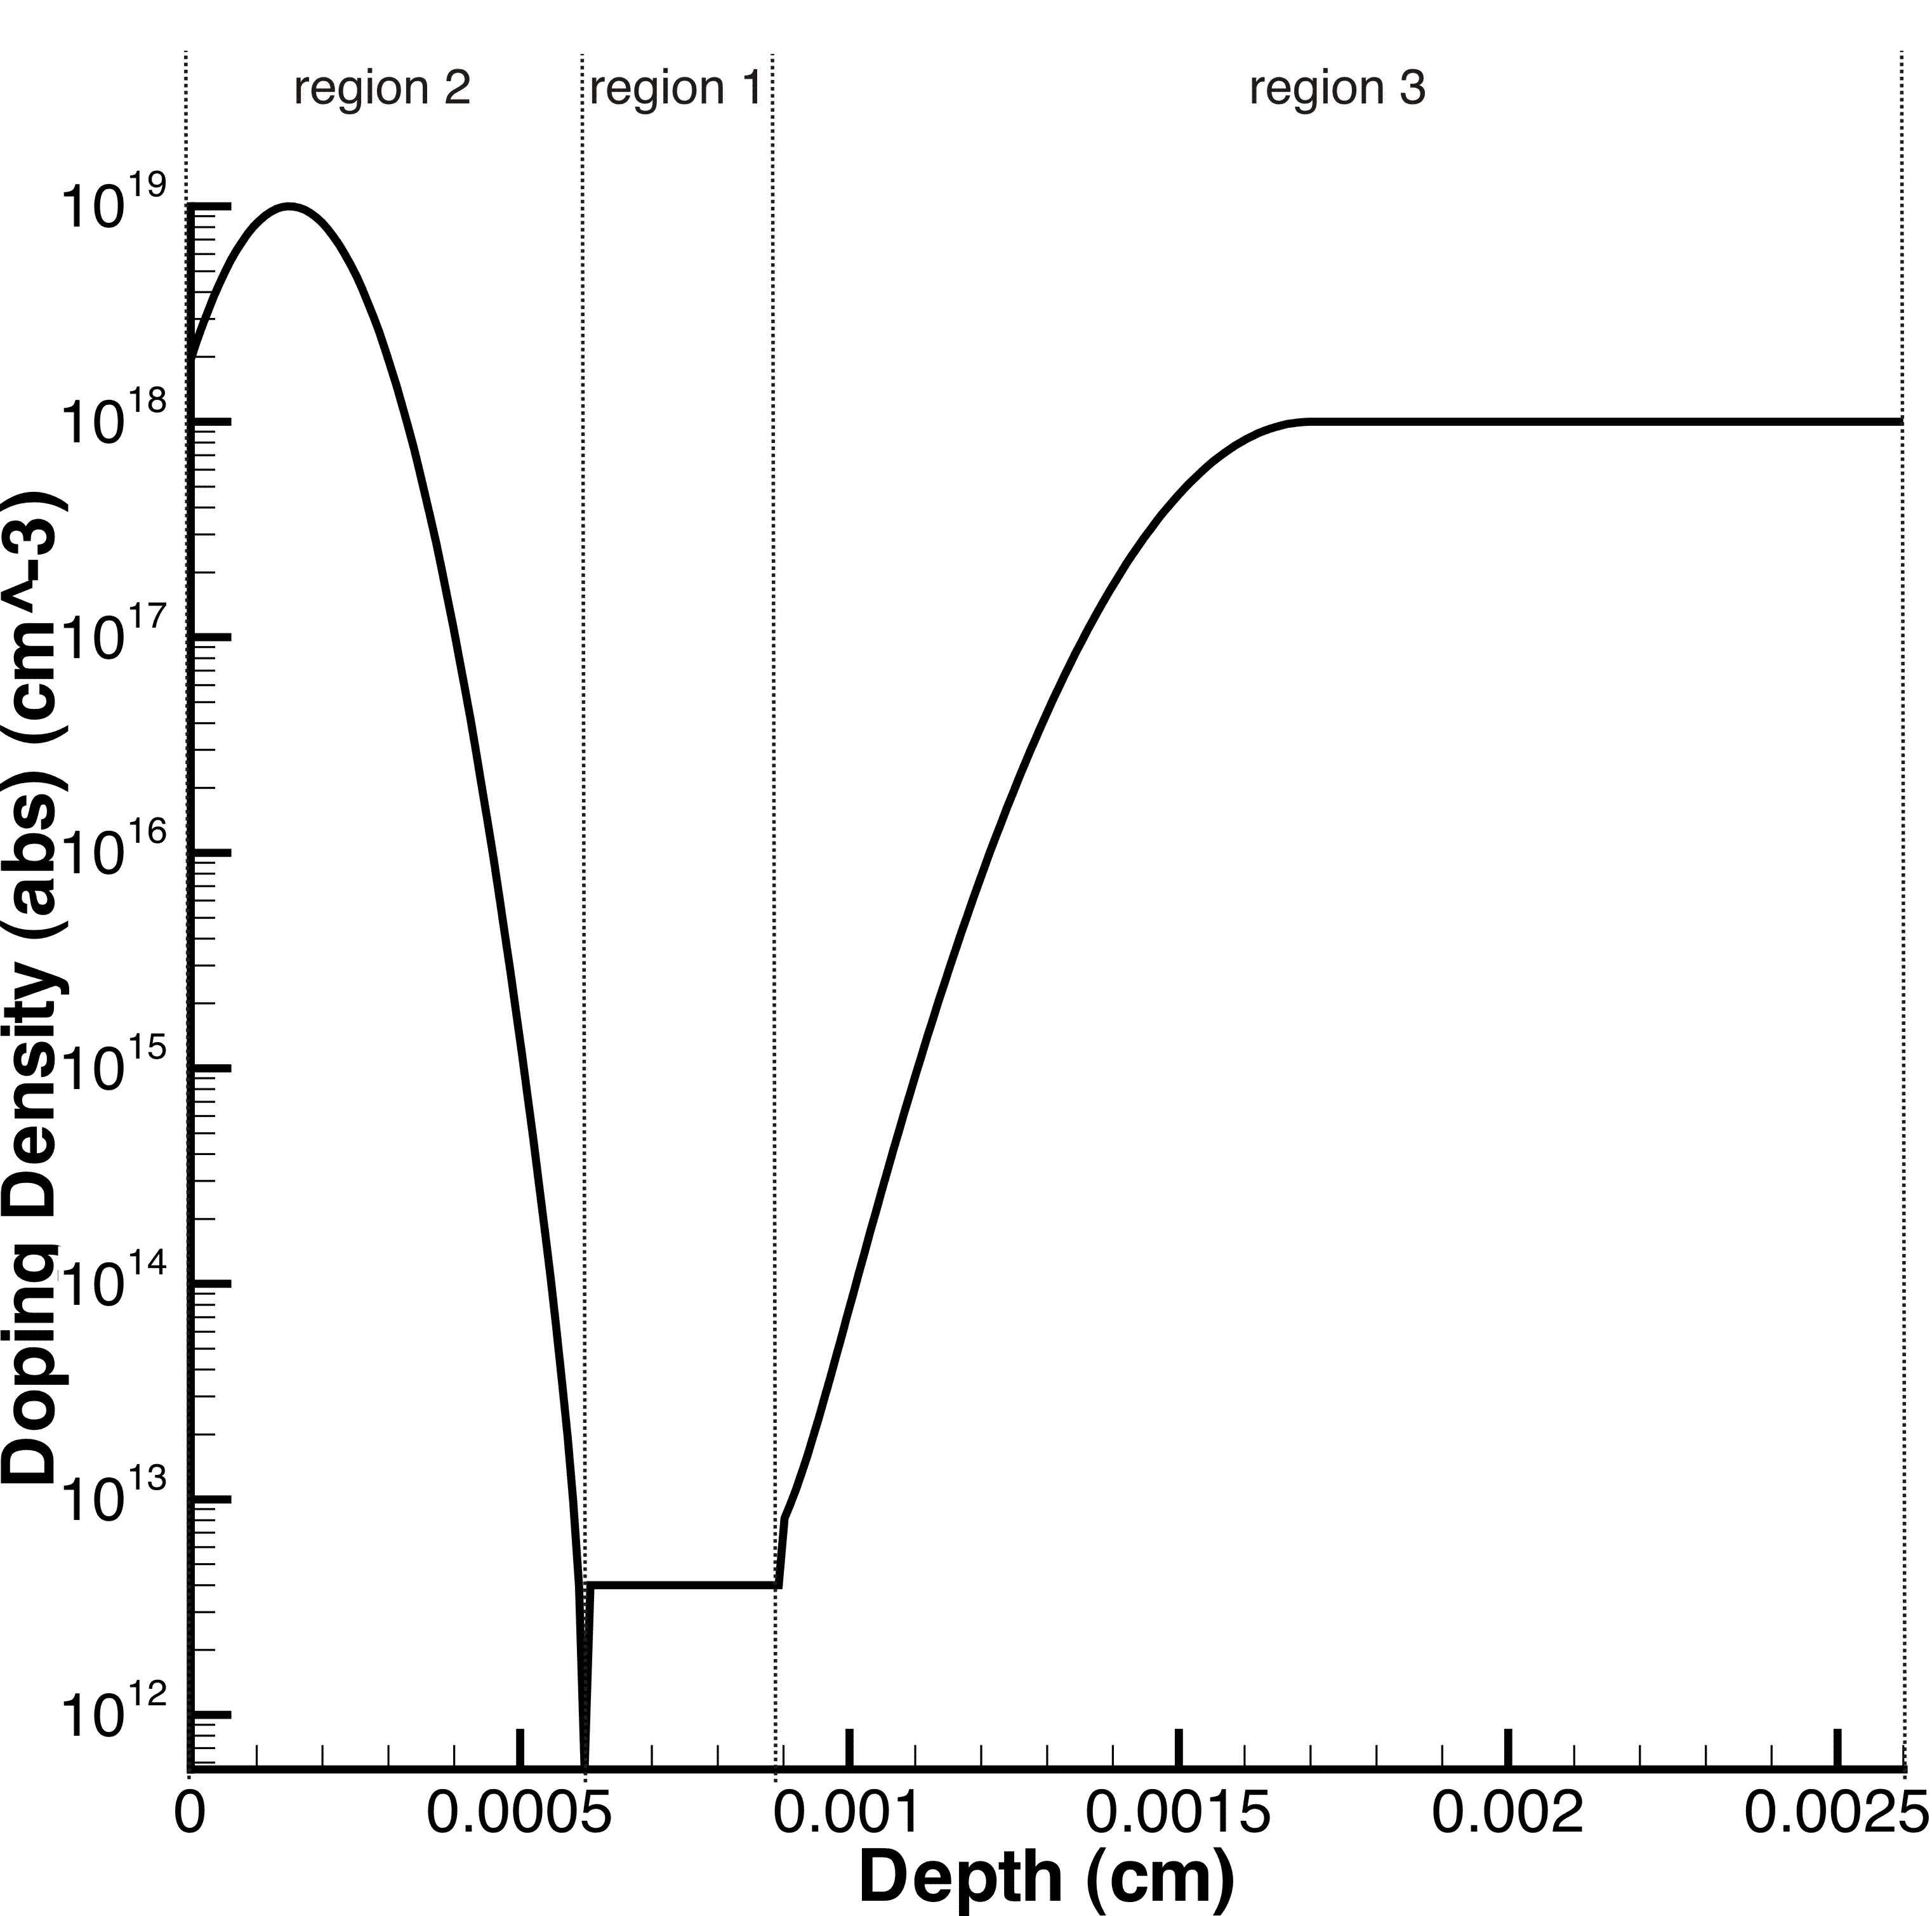
\includegraphics[width=4.610in,height= 4.45in]{doping_log}}
  \caption[Doping profile, absolute value]{Doping profile, absolute value  
This corresponds to the doping specified by the netlist in figure~\ref{One_D_Doping_Electrode_1}\label{Doping_Profile_1D}}
\end{figure}

Region 3 is also based on a Gaussian function, but unlike Region 2, it is 
flat on one side of the peak.  This is set by the \texttt{flatx} parameter.  
Table~\ref{flatxy_table} lists conventions for ``flat'' parameters.

\LTXtable{\textwidth}{flattbl}

%\include{expressionDoping}

\newpage
\subsection{Default Doping Profiles}
\Xyce{} has a few default doping profiles that are invoked when the user
doesn't specify detailed doping information.  The default doping 
profiles are an artifact of early TCAD device development in \Xyce{}, but are 
sometimes still useful.  In particular, the simple step-junction diode
is often a useful canonical problem.  It is convenient to invoke a
step-junction doping without having to use the tabular specification
for more complex regions.

Most real devices will have doping profiles that do not exactly match the
default profiles.  When attempting to simulate a realistic device, it
will be necessary to skip the defaults and use the region tables described in
the previous section.

\subsubsection{One-Dimensional Case} \label{one_d_default_dope}
For the one-dimensional case, \Xyce{} assumes that the doping profile is a
simple junction diode, with the junction location exactly in the middle.  The
acceptor and donor concentrations are given by the parameters \texttt{Na} and
\texttt{Nd}, respectively.  

The use of ~\texttt{Na} and \texttt{Nd}, implicitly specifies a step junction
doping profile, and is mutually exclusive with the more complex ``doping
region'' table specification, described in section~\ref{Manual_Doping}.  If a
netlist is input to \Xyce{} with a ``doping region'' table and \texttt{Na} (or
\texttt{Nd}), the code will immediately exit with an error.

\subsubsection{Two-Dimensional Case} \label{two_d_default_dope}
Doping level defaults in the two-dimensional case are somewhat more complicated
than in the one-dimensional case, because having two-dimensions allows for more
configurations, and an arbitrary number (2 to 4) of electrodes.  During \Xyce{}
development, it was decided that the default doping profiles would be
determined uniquely by the number of electrodes present.
Table~\ref{Default_Doping_2D} provides the three available default dopings.  In
the case of the BJT and MOSFET dopings, it is possible to specify either n-type
or p-type using the \texttt{type} instance parameter.   If the detailed, manual
doping is used, then the \texttt{type} parameter is ignored.

For a two-electrode device, the default doping is that of a simple diode.
\Xyce{} uses the acceptor and donor doping parameters, \texttt{Na} and
\texttt{Nd}, in the same manner as in the one-dimensional device---the junction
is assumed to be exactly in the middle of the domain.

For a three-electrode device (as shown in the example), the default doping is
that of a bipolar junction transistor (BJT).  By default the transistor is a
PNP, but by setting the instance parameter \texttt{type=NPN}, an NPN transistor
can be specified instead.  The two-dimensional example in
section~\ref{PDE_Two_D_Example} relies on this default.  

For a four-terminal device, the default doping is that of a
metal-oxide-semiconductor (MOSFET).  The maximum number of electrodes is four,
and no default profiles are available for more than four electrodes.  By
default this transistor is assumed to be NMOS, rather than PMOS.

\LTXtable{\textwidth}{defdopingtbl}

\clearpage
\section{Electrodes} \label{PDE_Electrode}
Because minimal electrodes were specified in the two examples given above, \Xyce{}
used the defaults.  In practice, especially for two-dimensional simulations, the 
user must specify the electrodes in more detail.

% electrode specification example.  
\begin{figure}
  \begin{centering}
    \shadowbox{
      \begin{minipage}{0.8\textwidth}
        \begin{vquote}

\color[gray]{0.5}Doping and electrode specification example
vscope   1   0   0.0
rscope   2   1   50.0
cid      3   0   1.0u
r1       4   3   1515.0
vid      4   0   1.00 \color{black}
*------------- Diode PDE device ------------------
YPDE Z1DIODE 2 3 PDEDIODE
+ tecplotlevel=1 txtdatalevel=1 cyl=1
+ meshfile=internal.msh 
+ nx=25  l=70.0e-4 ny=40  w=26.0e-4 
\color{XyceDarkBlue} * ELECTRODES:             ckt node 2, ckt node 3
+ node = \{name           =     anode,    cathode
+         bc             = dirichlet,  dirichlet
+         start          =     0.002, 0.002
+         end            =     0.005, 0.005
+         side           =       top,     bottom
+         material       =   neutral,    neutral
+         oxideBndryFlag =         0,          0 \}
\color{XyceRed}* DOPING REGIONS:    region 1,  region 2,   region 3
+ region= \{name    =     reg1,      reg2,  reg3
+          function = uniform,  gaussian, gaussian
+          type     =   ntype,     ptype,     ntype
+          nmax     = 4.0e+12,   1.0e+19,   1.0e+18
+          nmin     = 0.0e+00,   4.0e+12,   4.0e+12
+          xloc     =    0.0 ,  60.0e-04,    100.0 
+          xwidth   =    0.0 ,   4.0e-04,      1.0 
+          yloc     =    0.0 ,  24.5e-04,   9.0e-04
+          ywidth   =    0.0 ,   4.5e-04,   8.0e-04
+          flatx    =    0   ,       -1 ,       -1 
+          flaty    =    0   ,        0 ,       -1 \}\color{black}
*--------end of  Diode PDE device ----------------\color[gray]{0.5}
.MODEL PDEDIODE  ZOD  level=2 
.options NONLIN maxsearchstep=1 searchmethod=2 
.options TIMEINT reltol=1.0e-3 abstol=1.0e-6 
.DC vscope 0 0 1
.print DC v(1) v(2) v(3) v(4) I(vscope) I(vid)
.END
\end{vquote}
\end{minipage}
}
\caption{Two-dimensional example, with detailed doping and detailed electrodes.
\label{Two_D_Doping_Electrode_1}}
\end{centering}
\end{figure}

\subsection{Electrode Specification}
A detailed electrode specification is specified in blue text
in figure~\ref{Two_D_Doping_Electrode_1}.  As with the doping parameters, 
the electrode parameters are specified in a tabular format, in which each table 
column specifies the different electrode parameters.  The \texttt{name} parameter 
is the only required parameter.

The number of specified electrodes must match the number of connected 
circuit nodes, and the order of the electrode columns, from left to right,
is in the same order as the circuit nodes, also from left to right.  In 
the figure~\ref{Two_D_Doping_Electrode_1} example, the first electrode column,
which specifies an electrode named ``anode,'' is connected to the circuit 
through circuit node 2.  Respectively, the second column, for the ``cathode'' 
electrode, is connected to the circuit via circuit node 3.

\subsubsection{Boundary Conditions}
In the example, the default \texttt{bc} parameter has been set to ``Dirichlet''
on all the electrodes. The \texttt{bc} parameter sets the type of boundary 
condition applied to the density variables, the electron density and the hole density.
Dirichlet and Neumann are two possible settings for the \texttt{bc} parameter.  
If Dirichlet is specified, the electron and hole densities are set to a specific 
value at the contact, and the applied values enforce charge neutrality.  
(Note: The \Xyce{} Reference Guide\ReferenceGuide{} provides the charge-neutral 
equation.)  If Neumann is specified, \Xyce{} applies a zero-flux condition, 
which enforces that the current through the electrode will be zero.

This parameter does not affect the electrostatic potential boundary condition.
The boundary condition applied to the potential is always Dirichlet, and is
(in part) determined from the connected nodal voltage.  To apply a specific
voltage to an electrode contact, a voltage source should be attached to it,
such as \texttt{VBB} in figure~\ref{twoD_BJT_Schem}.

\subsubsection{Electrode Material}
Table~\ref{contactMaterialTable} lists several different electrode materials that can be specified.   
The main effect of any metal (nonneutral) material is that \Xyce{} imposes a
Schottky barrier at the contact, generally making numerical solutions
more difficult, so materials should be applied with caution.

The \Xyce{} Reference Guide\ReferenceGuide{}
provides a detailed description of Schottky barriers and how they are imposed on contacts in \Xyce{}.
The guide also provides values for electron affinities of various bulk materials and 
workfunction values for the various metal contacts.

\LTXtable{\textwidth}{contactMaterialtbl}

There is also an \texttt{oxideBndryFlag} parameter, which if set to true
(\texttt{1}), will model the contact as having an oxide layer in between
the metal contact and the bulk semiconductor.  By default,
\texttt{oxideBndryFlag} is false (\texttt{0}).  

\subsubsection{Location Parameters}
Each electrode has three location parameters: \texttt{start}, 
\texttt{end}, and \texttt{side}.  

\Xyce{} assumes the internal mesh to be rectangular, 
and the electrodes can be on any of the sides.  The four side possibilities
are: \texttt{top}, \texttt{bottom}, \texttt{right} and \texttt{left}.
These four sides are parallel to the mesh directions.  The \texttt{start} and
\texttt{end} parameters are floating-point numbers that specify the
starting and ending location of an electrode, in centimeters.

The lower left hand corner of the mesh rectangle is located 
at the origin.  A \texttt{side=bottom} electrode with \texttt{start=0.0} 
and \texttt{end=1.0e-4} will originate at the lower left hand 
corner of the mesh (x=0.0, y=0.0) and end at (x=1.0e-4, y=0.0).

\Xyce{} will attempt to match the specified electrode to
the specified mesh.  However, if the user specifies a mesh that is not
consistent with the electrode locations then the electrodes will not be 
able to have the exact length specified.  For example, if the mesh spacing
is $\Delta x = $ 1.0e-5, then the electrodes can only have a length
that is a multiple of 1.0e-5.

\subsection{Electrode Defaults}
Defaults exist for each electrode parameter other than names.
In practice, the electrode locations  are usually explicitly
specified  using the electrode table.
Default electrode locations were created to correspond with 
the default dopings; they should only be used in that context.

\subsubsection{Location Parameters}
In practice, the electrode locations will usually be explicitly
specified, but they have defaults to correspond with the default dopings.
The default electrode locations in one-dimensional devices are for a 
diode.  One electrode is located at \texttt{x=xmin}, while the other 
is located at \texttt{x=xmax}.

The default electrode locations in two-dimensional devices depend on the number 
of electrodes, similar to the default dopings.  Table~\ref{Default_Doping_2D} can be 
used to determine such configurations.  For the two-terminal diode, 
the two electrodes are along the  y-axis, at the \texttt{x=xmin} and 
\texttt{x=xmax} extrema.
For the three-terminal BJT, all three electrodes are parallel to the
x-axis, along the top, at \texttt{y=ymax}.  For the four-terminal MOSFET, the 
drain, gate, and source electrodes are also along the top, but the bulk 
electrode spans the entire length of the bottom of the mesh, at 
\texttt{y=ymin}.

\section{Meshes} \label{PDE_Mesh}
One- and two-dimensional devices can create Cartesian meshes.
For two-dimensional devices, users must specify \texttt{meshfile=internal.msh} 
to invoke the Cartesian meshing capability (this is necessary for historical reasons).
Meshes generated in this manner are very simple as there are only two
parameters per dimension, and the resulting mesh is uniform.  Figure~\ref{twoD_BJTResA} 
provides an example of such a mesh.  Mesh spacing is determined from the following expressions:
\begin{eqnarray}
  \Delta x = \frac{l}{nx-1}  \\
  \Delta y = \frac{w}{ny-1} 
\end{eqnarray}
This mesh specification assumes the domain is a rectangle.  
Nonrectangular domains can only be described using an external mesh program.

Externally generated meshes for 1D devices can be including using
\texttt{meshfile=<filename>} in the PDE device instance line. The file
specified by \texttt{<filename>} must consist of two space-delimited columns of
numbers. The first column specifies the location of the mesh points. The second
column is not currently used, but it must exist, so it is suggested to make it
a column of zeros.

\section{Cylindrical meshes}
For two-dimensional devices, the simulation area may be a cylinder slice.  
This capability is turned on by the instance parameter {\tt cyl=1} 
It is assumed that the
axis of the cylinder corresponds to the minimum radius (or x-axis value) of the 
mesh, while the circumference corresponds to the maximum radius (or maximum x-axis value).  

\section{Mobility Models}
\label{PDE_Mobility}
There are several mobility models available to the one- and two-dimensional 
devices, and they are listed in Table~\ref{Mobility_Models}.
These models are fairly common, and can be found in most device
simulators.~\cite{Yu}~\cite{DaVinci}. The \Xyce{} Reference 
Guide\ReferenceGuide{} descibes these models in more detail.

\LTXtable{\textwidth}{mobilitytbl}

Setting the {\texttt{mobmodel}} parameter to the name of the model (as provided 
in the first column of table~\ref{Mobility_Models}) specifies the mobility model 
from the netlist. The mobility model is specified as an instance parameter on the 
device instance line, as (typically) {\texttt {mobmodel=arora}}.
Figure~\ref{Two_D_BJT_Netlist} provides a more detailed 
example.

The default mobility is ``arora'', which is a basic model lacking carrier or field dependence.  
Because it lacks these dependencies, it generally is more numerically robust.  The ``carr'' model
include carrier-carrier dependence, as does the ``philips'' model.  For all of these models,
field dependence can be optionally turned on from the netlist, using the \texttt{fielddep=true} parameter.

\section{Bulk Materials}
\label{PDE_Bulk_Material}
The bulk material is specified using the \texttt{bulkmaterial} instance
parameter.  \Xyce{} supports Silicon (\texttt{si}) as a default bulk material.  
It can also simulate several III-V materials, including Gallium Arsenide (\texttt{gaas}), Germanium (\texttt{ge}), Indium Aluminum Arsenide (\texttt{inalas}  or \texttt{alinas}),
Indium Galium Arsenide (\texttt{ingaas} or \texttt{gainas}), Indium Phosphide(\texttt{inp}), and
Indium Galium Phosphide (\texttt{ingap}); but these materials have not been extensively tested.
The mobility models described in the previous section each support most of these materials.

\section{Output and Visualization}
\label{PDE_Output_Vis}

\subsection{Using the \texttt{.PRINT} Command }
For simple plots (such as I-V curves), output results for \Xyce{}
can be generated with the \texttt{.PRINT} statement, which is described in
detail in section~\ref{PRINT_section}.
Figures~\ref{One_D_outputSignal} and~\ref{twoD_BJTResC} are examples of
the kind of data that is produced with \texttt{.PRINT} statement
netlist commands.  These particular figures were plotted in Tecplot, but
many other plotting programs would also have worked, including
XDAMP~\cite{xdamp}.

\subsection{Multidimensional Plots}
Device simulation has visualization needs which go beyond that of 
conventional circuit simulation.  Multidimensional perspective and/or
contour plots are often desirable.  \Xyce{} is capable of outputting
multi-dimensional plot data in several formats, including Tecplot (available 
for purchase from http://www.tecplot.com), 
gnuplot (available free from http://www.gnuplot.info), and SGPLOT.
Currently, the options for each of these formats can only enable
or disable the output of files, and when enabled, a new file (or a new
append to an existing file) will happen at every time step or DC sweep
step.

For long simulations, this may produce a prohibitive number of files.  There is
no equivalent to the \texttt{.OPTIONS OUTPUT INITIAL\_INTERVAL} command, nor
does the output of plot data use this command.   Plot files are either output
at every step or not at all.

For each type of plot file, the file is placed in the execution directory.
Each individual device instance is given a unique file, or files, and
the file names are derived from the name of the PDE device instance.  The
instance names provides the prefix, and the file type (Tecplot,
gnuplot, Sgplot) determines the suffix.

\subsubsection{Tecplot Data}
Tecplot is a commercial plotting program from Amtec Engineering, Inc.,
and is a good choice for creating contour plots of spatially dependent
data.  All of the graphical examples in this chapter were created with
Tecplot. (See figures~\ref{twoD_BJTResA} and~\ref{twoD_BJTResB} for examples.)
The output of Tecplot files is enabled using the instance parameter,
\texttt{tecplotlevel=1}.  If set to zero, no Tecplot files are output.
If set to one, \Xyce{} outputs a separate Tecplot file for each nonlinear solve.
If set to two, \Xyce{} creates a single Tecplot file containing data for every 
nonlinear solve and appends the file at the end of each solve.

By default \texttt{tecplotlevel} is set to one, meaning the code will produce 
a separate Tecplot file for each time step or DC sweep step.   The
suffix for a Tecplot (ASCII text) data file is *.dat.

\subsubsection{Gnuplot Data}
Gnuplot is an open source plotting program available on most
Linux/Unix platforms.  The parameter for this type of output is 
\texttt{gnuplotlevel=1}.  This type of output file is off (zero) by 
default, meaning no gnuplot files will be output.  The suffix for gnuplot
files is *gnu.dat.  Like Tecplot files, gnuplot files are also in ASCII
text format.

\subsection{Additional Text Data}
\Xyce{} can also output additioanl information for each PDE device by setting 
the instance parameter, \texttt{txtdatalevel=1}.
It is on (1) by default, so this output will happen unless specifically disabled
by setting the parameter to zero.  A typical output file (associated with the
netlist given in figure~\ref{Two_D_BJT_Netlist}) is shown in figure~\ref{txtTwoD}.
\begin{figure}
  \begin{centering}
    \shadowbox{
      \begin{minipage}{0.8\textwidth}
        \begin{vquote}
Global data for DC step    1:
Current Time =   0.0000e+00
       Vmin  =  -8.6931e-06
       Vmax  =   5.4030e-01
       NnMin =   0.0000e+00
       NnMax =   1.0000e+16
       NpMin =   3.9240e+03
       NpMax =   1.0000e+19

Information for electrode: COLLECTOR
potential:   2.9795e-01
  current:   8.5365e-06
  charge:   -6.6211e-15
  dIdVckt:   3.7993e-02
  dQdVckt:   0.0000e+00

Information for electrode: BASE
potential:   5.4030e-01
  current:  -8.5408e-06
  charge:    1.5958e-14
  dIdVckt:   1.0463e+01
  dQdVckt:   0.0000e+00

Information for electrode: EMITTER
potential:  -8.6931e-06
  current:   4.3465e-09
  charge:   -2.3232e-13
  dIdVckt:   7.2130e+01
  dQdVckt:   0.0000e+00
\end{vquote}
\end{minipage}
}
\caption[Text output]
{Text output, from the circuit given in figure~\ref{Two_D_BJT_Netlist}.\label{txtTwoD}}
\end{centering}
\end{figure}


%%% Local Variables:
%%% mode: latex
%%% End:

%% END of Xyce_UG_PDE.tex ************
